\documentclass{article}

\newcommand{\dir}{~/projects/latex}
\input{\dir/include.tex}
\load{full}

\usepackage{lmodern}
% \usepackage{pgfplots}
\setFontType{sans}

\renewcommand{\authorTitle}{Robin Bacher, Janis Hutz\\\url{https://github.com/janishutz/eth-summaries}}
\renewcommand{\authorHeaders}{Robin Bacher, Janis Hutz}
\setLang{de}

\setup{Numerical Methods for Computer Science}

\begin{document}
\startDocument
\usetcolorboxes
\setcounter{numberingConfig}{3}
\setcounter{numberSubsections}{1}

%          ╭────────────────────────────────────────────────╮
%          │                   Title page                   │
%          ╰────────────────────────────────────────────────╯
\vspace{2cm}
\begin{Huge}
    \begin{center}
        TITLE PAGE COMING SOON
    \end{center}
\end{Huge}


\vspace{4cm}
\begin{center}
    \begin{Large}
        ``\textit{Denken vor Rechnen}''
    \end{Large}

    \hspace{3cm} - Vasile Grudinaru, 2025
\end{center}

\vspace{3cm}
\begin{center}
    HS2025, ETHZ\\[0.2cm]
    \begin{Large}
        Summary of the Script and Lectures
    \end{Large}\\[0.2cm]
\end{center}


% ────────────────────────────────────────────────────────────────────

%          ╭────────────────────────────────────────────────╮
%          │               Table of Contents                │
%          ╰────────────────────────────────────────────────╯
\newpage
\printtoc{ForestGreen}


% ────────────────────────────────────────────────────────────────────

%          ╭────────────────────────────────────────────────╮
%          │                  Introduction                  │
%          ╰────────────────────────────────────────────────╯
\newpage
\setcounter{section}{-1}
\section{Introduction}
This summary is intended to give you a broad overview of the topics relevant for the exam and is not intended to serve as a full on replacement for the script.
We have decided to write it in German, as is the new script and for some of the topics that are poorly explained in the script, we have added further explanations.

The numbering should match the script's numbering exactly (apart from the cases where two definitions were combined due to being closely related and short), making it easier for you to look up the relevant definitions, theorems, etc in context in the script.


% ────────────────────────────────────────────────────────────────────

%          ╭────────────────────────────────────────────────╮
%          │                  Main content                  │
%          ╰────────────────────────────────────────────────╯

% ── Introduction ────────────────────────────────────────────────────
\newsection
\section{Einführung}
% ┌                                                ┐
% │     AUTHOR: Janis Hutz<info@janishutz.com>     │
% └                                                ┘

\subsection{Rundungsfehler}

\begin{definition}[]{Absoluter \& Relativer Fehler}
    \begin{multicols}{2}
        \begin{itemize}
            \item \bi{Absoluter Fehler}: $||\tilde{x} - x||$
            \item \bi{Relativer Fehler}: $\displaystyle \frac{||\tilde{x} - x||}{||x||}$ für $||x|| \neq 0$
        \end{itemize}
    \end{multicols}
    wobei $\tilde{x}$ eine Approximation an $x \in \R$ ist
\end{definition}

Rundungsfehler entstehen durch die (verhältnismässig) geringe Präzision die man mit der Darstellung von Zahlen auf Computern erreichen kann.
Zusätzlich kommt hinzu, dass durch Unterläufe (in diesem Kurs ist dies eine Zahl die zwischen $0$ und der kleinsten darstellbaren, positiven Zahl liegt) Präzision verloren gehen kann.

Überläufe hingegen sind konventionell definiert, also eine Zahl, die zu gross ist und nicht mehr dargestellt werden kann.


\setLabelNumber{all}{9}
\begin{remark}[]{Auslöschung}
    Bei der Subtraktion von zwei ähnlich grossen Zahlen kann es zu einer Addition der Fehler der beiden Zahlen kommen, was dann den relativen Fehler um einen sehr grossen Faktor vergrössert.
    Die Subtraktion selbst hat einen vernachlässigbaren Fehler
\end{remark}

\setLabelNumber{all}{18}
\fancyex{Ableitung mit imaginärem Schritt} Als Referenz in Graphen wird hier oftmals die Implementation des Differenzialquotienten verwendet.

Der Trick hier ist, dass wir mit Komplexen Zahlen in der Taylor-Approximation einer glatten Funktion in $x_0$ einen rein imaginären Schritt durchführen können:
\begin{align*}
    f(x_0 + ih) = f(x_0) + f'(x_0)ih - \frac{1}{2} f''(x_0)h^2 - iC \cdot h^3 \text{ für } h \in \R \text{ und } h \rightarrow 0
\end{align*}
Da $f(x_0)$ und $f''(x_0)h^2$ reell sind, verschwinden die Terme, wenn wir nur den Imaginärteil des Ausdruckes weiterverwenden. Nach weiteren Vereinfachungen und Umwandlungen erhalten wir
\begin{align*}
    f'(x_0) \approx \frac{\text{Im}(f(x_0 + ih))}{h}
\end{align*}

Falls jedoch hier die Auswertung von $\text{Im}(f(x_0 + ih))$ nicht exakt ist, so kann der Fehler beträchtlich sein.


\setLabelNumber{all}{20}
\fancyex{Konvergenzbeschleunigung nach Richardson}
\begin{align*}
    y f'(x) & = y d\left(\frac{h}{2}\right) + \frac{1}{6} f'''(x) h^2 + \frac{1}{480}f^{(s)} h^4 + \ldots - f'(x) \\
            & = -d(h) - \frac{1}{6}f'''(x) h^2 + \frac{1}{120} f^{(s)}(x) h^n \Leftrightarrow 3 f'(x)             \\
            & = 4 d\left(\frac{h}{2}\right)  d(h) + \tco{h^4} \Leftrightarrow
\end{align*}
% TODO: Need to finish with notes from the exercise sessions


\fhlc{Cyan}{Schema}

\begin{align*}
    d(h) = \frac{f(x + h) - f(x - h)}{2h}
\end{align*}

wobei im Schema dann
\begin{align*}
    R_{l, 0} = d\left( \frac{h}{2^l} \right)
\end{align*}
und
\begin{align*}
    R_{l, k} = \frac{4^k \cdot R_{l, k - 1} - R_{l - 1, k - 1}}{4^k - 1}
\end{align*}
und $f'(x) = R_{l, k} + C \cdot \left( \frac{h}{2^l} \right)^{2k + 2}$

\newsection
\subsection{Rechenaufwand}
In NumCS wird die Anzahl elementarer Operationen wie Addition, Multiplikation, etc benutzt, um den Rechenaufwand zu beschreiben. 
Wie in Algorithmen und * ist auch hier wieder $\tco{\ldots}$ der Worst Case.
Teilweise werden auch andere Funktionen wie $\sin, \cos, \sqrt{\ldots}, \ldots$ dazu gezählt.

Die Basic Linear Algebra Subprograms (= BLAS), also grundlegende Operationen der Linearen Algebra, wurden bereits stark optimiert und sollten wann immer möglich verwendet werden und man sollte auf keinen Fall diese selbst implementieren.

Dieser Kurs verwendet \texttt{numpy}, \texttt{scipy}, \texttt{sympy} (collection of implementations for symbolic computations) und \texttt{matplotlib}.
Dieses Ecosystem ist eine der Stärken von Python und ist interessanterweise zu einem Grossteil nicht in Python geschrieben, da dies sehr langsam wäre.

\newsection
\subsection{Rechnen mit Matrizen}
Wie in Lineare Algebra besprochen, ist das Resultat der Multiplikation einer Matrix $A \in \C^{m \times n}$ und einer Matrix $B \in \C^{n \times p}$ ist eine Matrix $AB = \in \C^{m \times p}$

\fhlc{Cyan}{In NumPy} haben wir folgende Funktionen:
\begin{itemize}
    \item \verb|b @ a| (oder \verb|np.dot(b, a)| oder \verb|np.einsum('i,i', b, a)| für das Skalarprodukt
    \item \verb|A @ B| (oder \verb|np.einsum('ik,kj->ij', )|) für das Matrixprodukt
    \item \verb|A @ x| (oder \verb|np.einsum('ij,j->i', A, x)|) für Matrix $\times$ Vektor
    \item \verb|A.T| für die Transponierung
    \item \verb|A.conj()| für die komplexe Konjugation (kombiniert mit \verb|.T| = Hermitian Transpose)
    \item \verb|np.kron(A, B)| für das Kroneker Produkt
    \item \verb|b = np.array([4.j, 5.j])| um einen Array mit komplexen Zahlen zu erstellen (\verb|j| ist die imaginäre Einheit, aber es muss eine Zahl direkt daran geschrieben werden)
\end{itemize}


\setcounter{all}{4}
\fancyremark{Rang der Matrixmultiplikation} $\text{Rang}(AX) = \min(\text{Rang}(A), \text{Rang}(X))$

\setcounter{all}{7}
\fancyremark{Multiplikation mit Diagonalmatrix $D$} $D \times A$ skaliert die Zeilen von $A$ während $A \times D$ die Spalten skaliert

\stepcounter{all}
\inlineex \verb|D @ A| braucht $\tco{n^3}$ Operationen, wenn wir jedoch \verb|D.diagonal()[:, np.newaxis] * A| verwenden, so haben wir nur noch $\tco{n^2}$ Operationen, da wir die vorige Bemerkung Nutzen und also nur noch eine Skalierung vornehmen.
So können wir also eine ganze Menge an Speicherzugriffen sparen, was das Ganze bedeutend effizienter macht

\setcounter{all}{14}
\inlineremark Wir können bestimmte Zeilen oder Spalten einer Matrix skalieren, in dem wir einer Identitätsmatrix im unteren Dreieck ein Element hinzufügen.
Wenn wir nun diese Matrix $E$ (wie die in der $LU$-Zerlegung) linksseitig mit der Matrix $A$ multiplizieren (bspw. $E^{(2, 1)}A$), dann wird die zugehörige Zeile skaliert.
Falls wir aber $AE^{(2, 1)}$ berechnen, so skalieren wir die Spalte

\fancyremark{Blockweise Berechnung} Man kann das Matrixprodukt auch Blockweise berechnen.
Dazu benutzen wir eine Matrix, deren Elemente andere Matrizen sind, um grössere Matrizen zu generieren.
Die Matrixmultiplikation funktioniert dann genau gleich, nur dass wir für die Elemente Matrizen und nicht Skalare haben.

% ────────────────────────────────────────────────────────────────────
\hspace{1mm}
\hrule
\hspace{1mm}
Untenstehend eine Tabelle zum Vergleich der Operationen auf Matrizen

\begin{tables}{lcccc}{Name           & Operation & Mult  & Add         & Komplexität}
              Skalarprodukt          & $x^H y$   & $n$   & $n - 1$     & $\tco{n}$    \\
              Tensorprodukt          & $x y^H$   & $nm$  & $0$         & $\tco{mn}$   \\
              Matrix $\times$ Vektor & $Ax$      & $mn$  & $(n - 1)m$  & $\tco{mn}$   \\
              Matrixprodukt          & $AB$      & $mnp$ & $(n - 1)mp$ & $\tco{mnp}$  \\
\end{tables}
\inlineremark Das Matrixprodukt kann mit Strassen's Algorithmus mithilfe der Block-Partitionierung in $\tco{n^{\log_2(7)}} \approx \tco{n^{2.81}}$ berechnet werden.

\fancyremark{Rang 1 Matrizen} Können als Tensorprodukt von zwei Vektoren geschrieben werden.
Dies ist beispielsweise hierzu nützlich:

Sei $A = ab^\top$. Dann gilt $y = Ax \Leftrightarrow y = a(b^\top x)$, was dasselbe Resultat ergibt, aber nur $\tco{m + n}$ Operationen und nicht $\tco{mn}$ benötigt wie links.

\inlineex Für zwei Matrizen $A, B \in \R^{n \times p}$ mit geringem Rang $p \ll n$, dann kann mithilfe eines Tricks die Rechenzeit von \verb|np.triu(A @ B.T) @ x| von $\tco{pn^2}$ auf $\tco{pn}$ reduziert werden.
Die hier beschriebene Operation berechnet $\text{Upper}(AB^\top) x$ wobei $\text{Upper}(X)$ das obere Dreieck der Matrix $X$ zurück gibt.
Wir nennen diese Matrix hier $R$.
Wir können in NumPy den folgenden Ansatz verwenden, um die Laufzeit zu verringern:
Da die Matrix $R$ eine obere Dreiecksmatrix ist, ist das Ergebnis die Teilsummen von unserem Umgekehrten Vektor $x$, also können wir mit \verb|np.cumsum(x[::-1], axis=0)[::-1]| die Kummulative Summe berechnen.
Das \verb|[::-1]| dient hier lediglich dazu, den Vektor $x$ umzudrehen, sodass das richtige Resultat entsteht.
Die vollständige Implementation sieht so aus:
\begin{minted}{python}
import numpy as np

def low_rank_matrix_vector_product(A: np.ndarray, B: np.ndarray, x: np.ndarray):
    n, _ = A.shape
    y = np.zeros(n)

    # Compute B * x with broadcasting (x needs to be reshaped to 2D)
    v = B * x[:, None]

    # s is defined as the reverse cummulative sum of our vector
    # (and we need it reversed again for the final calculation to be correct)
    s = np.cumsum(v[::-1], axis=0)[::-1]

    y = np.sum(A * s)
\end{minted}


\setcounter{all}{21}
\fancydef{Kronecker-Produkt} Das Kronecker-Produkt ist eine $(ml) \times (nk)$-Matrix, für $A \in \R^{m \times n}$ und $B \in \R^{l \times k}$, die wir in NumPy einfach mit \verb|np.kron(A, B)| berechnen können (ist jedoch nicht immer ideal):
\begin{align*}
    A \otimes B :=
    \begin{bmatrix}
        (A)_{1, 1} B & (A)_{1, 2}B & \ldots & \ldots & (A)_{1, n} B \\
        (A)_{2, 1} B & (A)_{2, 2}B & \ldots & \ldots & (A)_{2, n} B \\
        \vdots       & \vdots      & \ddots & \ddots & \vdots       \\
        (A)_{m, 1} B & (A)_{m, 2}B & \ldots & \ldots & (A)_{m, n} B \\
    \end{bmatrix}
\end{align*}

\fancyex{Multiplikation des Kronecker-Produkts mit Vektor} Wenn man $A \otimes B \cdot x$ berechnet, so ist die Laufzeit $\tco{m \times n \times l \times k}$, aber wenn wir den Vektor $x$ in $n$ gleich grosse Blöcke aufteilen (was man je nach gewünschter nachfolgender Operation in NumPy in $\tco{1}$ machen kann mit \verb|x.reshape(n, x.shape[0] / n)|), dann ist es möglich das Ganze in $\tco{m \cdot l \cdot k}$ zu berechnen. 

Die vollständige Implementation ist auch hier nicht schwer und sieht folgendermassen aus:
\begin{minted}{python}
import numpy as np

def fast_kron_vector_product(A: np.ndarray, B: np.ndarray, x: np.ndarray):
    # First multiply Bx_i, (and define x_i as a reshaped numpy array to save cost (as that will create a valid array))
    # This will actually crash if x.shape[0] is not divisible by A.shape[0]
    bx = B * x.reshape(A.shape[0], round(x.shape[0] / A.shape[0]))
    # Then multiply a with the resulting vector
    y = A * bx
\end{minted}

Um die oben erwähnte Laufzeit zu erreichen muss erst ein neuer Vektor berechnet werden, oben im Code \verb|bx| genannt, der eine Multiplikation von \verb|Bx_i| als Einträge hat.


% ── polynomial interpolation ────────────────────────────────────────
\newsection
\section{Polynominterpolation}
\stepcounter{subsection}
\subsection{Continuity}
\compactdef{Convergence in $\R^n$} Let $(x_k)_{k \in \N}$ where $x_k \in \R^n$ with $x_k = (x_{k, 1}, \ldots, x_{k, n})$ and let $y = (y_1, \ldots, y_n) \in \R^n$.
$(x_k)$ converges to $y$ as $k \rightarrow +\infty$ if $\forall \varepsilon > 0 \smallhspace \exists N \geq 1$ s.t. $\forall n \geq N$ we have $||x_k - y|| < \varepsilon$
% ────────────────────────────────────────────────────────────────────
\shortlemma $(x_k)$ converges to $y$ as $k \rightarrow +\infty$ iff one of following equiv. statements holds:
\bi{(1)} $\forall 1 \leq i \leq n$, the sequence $(x_{k, i})$ with $x_{k, i} \in \R$ converges to $y_i$
\bi{(2)} $(||x_k - y||)$ converges to $0$ as $k \rightarrow +\infty$
% ────────────────────────────────────────────────────────────────────
\compactdef{Continuity} Let $X \subseteq \R^n$ and $f: X \rightarrow \R^m$.
\bi{(1)} Let $x_0 \in X$. $f$ continuous in $\R^n$ if $\forall \varepsilon > 0 \smallhspace \exists \delta > 0$ s.t. if $x \in X$ satisfies $||x - x_0|| < \delta$,
then $||f(x) - f(x_0)|| < \varepsilon$
\bi{(2)} $f$ continuous \textit{on} $X$ if continuous at $x_0 \smallhspace \forall x_0 \in X$
% ────────────────────────────────────────────────────────────────────
\shortproposition Let $X$ and $f$ as prev. Let $x_0 \in X$. $f$ continuous at $x_0$ iff $\forall (x_k)_{k \geq 1}$ in $X$ s.t.
$x_k \rightarrow x_0$ as $k \rightarrow +\infty$, $(f(x_k))_{k \geq 1}$ in $\R^m$ converges to $f(x)$\\
% ────────────────────────────────────────────────────────────────────
\compactdef{Limit} Let $X$, $f$ and $x_0$ as prev. and $y \in \R^m$. $f$ \textit{has limit} $y$ as $x \rightarrow x_0$ with $x \neq x_0$ if
$\forall \varepsilon > 0 \smallhspace \exists \delta > 0$ s.t. $\forall x \neq x_0 \in X, ||x - x_0|| < \delta$ we have $||f(x) - y|| < \varepsilon$.
We write $\lim_{\elementstack{x \rightarrow x_0}{x \neq x_0}} f(x) = y$
\shortremark Also possible without ass. that $x_0 \in X$
% ────────────────────────────────────────────────────────────────────
\shortproposition Let $X$, $f$, $x_0$ and $y$ as prev. We have $\lim_{\elementstack{x \rightarrow x_0}{x \neq x_0}} f(x) = y$ 
iff $\forall (x_k)$ in $X$ s.t. $x_k \rightarrow x$ as $k \rightarrow +\infty$ and $x_k \neq x_0$ $(f(x_k))$ in $\R^m$ converges to $y$
\stepLabelNumber{all}
\shortproposition Let $X \subseteq \R^n$, $y \subseteq \R^m$, $p \in \N$ and let $f: X \rightarrow Y$ and $g: Y \rightarrow \R^p$ be cont. Then $g \circ f$ is continuous

\subsubsection{Monombasis}

\fancytheorem{Eindeutigkeit} $p(x) \in \mathcal(P)_k$ ist durch $k+1$ Punkte $y_i = p(x_i)$ eindeutig bestimmt.

Dieser Satz kann direkt angewendet werden zur Interpolation, in dem man $p(x)$ als Gleichungssystem schreibt.
% FIXME: It'd probably be better to use align* environment in general, it's much more flexible
% FIXME: Having a new line before $$ (or align* environment for that matter) makes the space between text and math env larger!
$$
	p_n(x) = \alpha_n x^n + \cdots + \alpha_0 x^0 \quad \iff \quad
	\underbrace{
		\begin{bmatrix}
			1      & x_0    & \cdots & x_0^n  \\
			1      & x_1    & \cdots & x_1^n  \\
			\vdots & \vdots & \ddots & \vdots \\
			1      & x_n    & \cdots & x_n^n  \\
		\end{bmatrix}
	}_\text{Vandermonde Matrix}
	\begin{bmatrix}
		\alpha_0 \\
		\alpha_1 \\
		\vdots   \\
		\alpha_n
	\end{bmatrix}
	=
	\begin{bmatrix}
		y_0    \\
		y_1    \\
		\vdots \\
		y_n
	\end{bmatrix}
$$

Um $\alpha_i$ zu finden ist die Vandermonde Matrix unbrauchbar, da die Matrix schlecht konditioniert ist.

Zur Auswertung von $p(x)$ kann man direkt die Matrix-darstellung nutzen, oder effizienter:

\fancydef{Horner Schema} $p(x) = (x \ldots x ( x (\alpha_n x + \alpha_{n-1}) + \ldots + \alpha_1) + \alpha_0)$

\fhlc{Cyan}{In NumPy} \verb|polyfit| liefert die direkte Auswertung, \verb|polyval| wertet Polynome via Horner-Schema aus. (Gemäss Script, in der Praxis sind diese Funktionen \verb|deprecated|)

\newpage
\subsection{Newton Basis}
% Session: Herleitung unwichtig, konzentrieren auf Funktion/Eigenschaften von Newton/Lagrange.

Die Newton-Basis hat den Vorteil, dass sie leichter erweiterbar als die Monombasis ist.

Die Konstruktion verläuft iterativ, und vorherige Datenpunkte müssen nicht neuberechnet werden.

\begin{align*}
    p_0(x) &= y_0 &\textit{(Anfang: triviales Polynom)} \\
    p_1(x) &= p_0(x) + (x-x_0)\frac{(y_1-y_0)}{(x_1-x_0)} & \textit{(Addition des zweiten Datenpunktes)} \\
    p_2(x) &= p_1(x) + \frac{\frac{(y_2-y_1)}{(x_2-x_1)}-\frac{(y_1-y_0)}{x_1-x_0}}{x_2-x_0} (x-x_0)(x-x_1) & \textit{(Schema lässt sich beliebig weiterführen)}\\
    p_3(x) &= p_2(x) + \ldots
\end{align*}

\setcounter{all}{3}
\fancytheorem{Newton-Basis} $\{ N_0,\ \ldots\ ,N_n\}$ ist eine Basis von $\mathcal{P}_n$
\begin{align*}
    N_0(x) &:= 1 \quad
    N_1(x) := x - x_0 \quad
    N_2(x) := (x-x_0)(x-x_1) \quad \ldots \\
    N_n(x) &:= \prod_{i=0}^{n-1} (x-x_i)
\end{align*}

\subsubsection{Koeffizienten}

Wegen Satz 2.2.3 lässt sich jedes $p_n \in \mathcal{P}_n$ als $p_n(x) =\displaystyle\sum_{i=0}^{n} \beta_i N_i(x)$ darstellen. Ein Gleichungssystem liefert alle $\beta_i$:
\begin{align*}
    \begin{bmatrix}
        1 & 0   & \cdots & 0 \\
        1 & N_0 & \cdots & 0 \\
        \vdots & \vdots & \ddots & \vdots \\
        1 & N_0 & \cdots & N_n
    \end{bmatrix}
    \begin{bmatrix}
        \beta_0 \\
        \beta_1 \\
        \vdots \\
        \beta_n
    \end{bmatrix}
    =
    \begin{bmatrix}
        y_0 \\
        y_1 \\
        \vdots \\
        y_n
    \end{bmatrix}
\end{align*}

Die Matrixmultiplikation in $\mathcal{O}(n^3)$ ist aber nicht nötig: Es gibt ein effizienteres System. 

\setcounter{all}{5}
\fancydef{Dividierte Differenzen} 
\begin{multicols}{2}
    \begin{align*}
        y[x_i] &:= y_i \\
        y[x_i,\ \ldots\ ,x_{i+k}] &\overset{\text{Rec.}}{:=} \frac{y[x_{i+1},\ \ldots\ , x_{i+k}] - y[x_i,\ \ldots\ , x_{i+k-1}]}{x_{i+k}-x_i}
    \end{align*}

    \newcolumn

    \begin{center}
    \begin{tabular}{l|llll}
        $x_0$ & $y[x_0]$ \\
            &          & $>y[x_0,x_1]$        \\
        $x_1$ & $y[x_1]$ &  & $>y[x_0,x_1,x_2]$ \\ 
            &          & $>y[x_1,x_2]$        \\
        $x_2$ & $y[x_2]$ &  & $>y[x_1,x_2,x_3]$ \\
            &          & $>y[x_2,x_3]$        \\
        $x_3$ & $y[x_3]$                        \\
    \end{tabular}
    \end{center}
\end{multicols}

\fancyremark{Äquidistante Stellen}

Falls $x_j = x_0 + \underbrace{j \cdot h}_{:= \Delta^j}$ gilt vereinfacht sich einiges:
\begin{align*}
    y[x_0,x_1] &= \frac{1}{h}\Delta y_0 \\
    y[x_0,x_1,x_2] &= \frac{1}{2!h} \Delta^2 y_0 \\
    y[x_0,\ \ldots\ , x_n] &= \frac{1}{n! h^n} \Delta^n y_0 
\end{align*}

\setcounter{all}{8}
\fancytheorem{Newton} Falls $\beta_j = y[x_0,\ \ldots\ , x_j]$ geht das resultierende Polynom durch alle $(x_i,y_i)$.\\
\footnotesize
(D.h. die dividierten Differenzen sind korrekt.)
\normalsize

\fancyex{Runge-Funktion} Die Runge-Funktion kann am Rand des gewählten Intervalls starke Oszillationen in der Interpolation verursachen, 
wenn bspw. die Stützstellen nicht gut gewählt sind oder das Polynom einen zu hohen Grad hat.
Sie ist definiert durch $\displaystyle f(x) = \frac{1}{1 + x^2}$


\newpage
\begin{multicols}{2}

    Matrixmultiplikation in $\mathcal{O}(n^3)$, Speicher $\mathcal{O}(n^2)$

    \begin{code}{python}
    # Slow matrix approach
    def divdiff_slow(x,y):
        n = y.size
        T = np.zeros((n,n))
        T[:,0] = y

        for l in range(1,n):
            for i in range(n-l):
                T[i, l] = (T[i+1,l-1] - T[i, l-1])
                T[i, l] /= (x[i+l] - x[i])
        
        return T[0,:]
    \end{code}

    \newcolumn

    % Add the vectorized HW solution here

    Vektorisierter Ansatz in $\mathcal{O}(n^2)$, Speicher $\mathcal{O}(n)$

    \begin{code}{python}
    # Fast vectorized approach
    def divdiff_fast(x,y):
        n = y.shape[0]

        for k in range(1, n):
            y[k:] = (y[k:] - y[(k-1):n-1]) 
            y[k:] /= (x[k:] - x[0:n-k])
    
        return y
    \end{code}

\end{multicols}

\subsubsection{Auswertung}

Auswertung eines Newton-Polynoms funktioniert in $\mathcal{O}(n)$ durch ein modifiziertes Horner-Schema:

\begin{multicols}{2}
    
\begin{align*}
    p_0 &:= \beta_n \\
    p_1 &:= (x - x_{n-1})p_0 + \beta_{n-1} \\
    p_2 &:= (x - x_{n-2})p_1 + \beta_{n-2} \\
    \vdots \\
    p_n &= p(x)
\end{align*}

\newcolumn

\begin{code}{python}
    def evalNewton(x_data, beta, x):
        p = np.zeros(x.shape[0])
        p += beta[beta.shape[0]-1]
    
        for i in range(1, n+1):
            p = (x - x_data[n-i])*p + beta[n-i]
      
        return p
\end{code}

\end{multicols}


\subsubsection{Fehler}

\setcounter{all}{11}
\inlinetheorem $f$ $n$-mal diff.-bar, $y_i = f(x_i) \implies \exists \xi \in (\min_i x_i, \max_i x_i)$ s.d. $y[x_0,x_1,\ldots,x_n] = \frac{f^{(n)}(\xi)}{(n+1)!}$

\fancytheorem{Fehler} $f: [a,b] \to \R$ ist $(n+1)$-mal diff.-bar, $p$ ist das Polynom zu $f$ in $x_0,\ldots,x_n \in [a,b]$. 
$$
    \forall x \in [a,b]\ \exists \xi \in (a,b):\quad\quad \underbrace{f(x)-p(x)}_{\text{Fehler}} = \prod_{i=0}^{n}(x-x_i)\cdot\frac{f^{(n+1)}(\xi)}{(n+1)!}
$$

Man bemerke: Die Wahl der Stützpunkte hat direkten Einfluss auf den Fehler.



% ┌                                                ┐
% │     AUTHOR: Janis Hutz<info@janishutz.com>     │
% └                                                ┘

\newsection
\subsection{Lagrange- und Baryzentrische Interpolationsformeln}
% Session: Gemäss TA sehr gut beschrieben im alten Script
\label{sec:barycentric-interpolation}

\begin{definition}[]{Lagrange Polynome}
    Für Knoten (auch gennannt Stützstellen) $x_0, x_1, \ldots, x_n \in \R$ definieren wir die Lagrange-Polynome für $n = \text{Anzahl Stützstellen}$, also haben wir $n - 1$ Brüche, da wir eine Iteration überspringen, weil bei dieser $j = i$ ist:
    \begin{align*}
        l_i(x) = \prod_{\elementstack{j = 0}{j \neq i}}^n \frac{x - x_j}{x_i - x_j}
    \end{align*}
\end{definition}
Falls $j = i$ im Produkt, so überspringt $j$ diese Zahl.

\inlineex Seien $x_0, x_1, x_2$ die Stützstellen für die Lagrange-Polynome (mit $n = 2$):
\begin{align*}
    l_0(x) & = \frac{x - x_1}{x_0 - x_1} \cdot \frac{x - x_2}{x_0 - x_2} &
    l_1(x) & = \frac{x - x_0}{x_1 - x_0} \cdot \frac{x - x_2}{x_1 - x_2} &
    l_2(x) & = \frac{x - x_0}{x_2 - x_0} \cdot \frac{x - x_1}{x_2 - x_1}
\end{align*}


\begin{theorem}[]{Lagrange-Interpolationsformel}
    Die Lagrange-Polynome $l_i$ zu den Stützstellen $(x_0, y_0), \ldots, (x_n, y_n)$ bilden eine Basis der Polynome $\mathcal{P}_n$ und es gilt:
    \begin{align*}
        p(x) = \sum_{i = 0}^{n} y_i l_i(x) \text{ mit } l_i(x) = \prod_{j \neq i} \frac{x - x_j}{x_i - x_j}
    \end{align*}
\end{theorem}


\fancyremark{Eigenschaften der Lagrange-Polynome}
\rmvspace
\begin{multicols}{2}
    \begin{enumerate}
        \item $l_i(x_j) = 0 \smallhspace \forall j \neq i$
        \item $l_i(x_i) = 1 \smallhspace \forall i$
        \item $\deg(l_i) = n \smallhspace \forall i$
        \item $\sum_{k = 0}^{n} l_k(x) = 1 \text{ und } \sum_{k = 0}^{n} l_k^{(m)}(x) = 0 \text{ für } m > 0$
    \end{enumerate}
\end{multicols}

Da eine Implementation, welche direkt auf den Lagrange-Polynomen basiert, eine Laufzeit von $\tco{n^3}$ hätte, suchte man nach einer besseren Methode.
Mit der \bi{baryzentrischen Interpolationsformel} wird zuerst ein Pre-Computing auf Teilen der Lagrange-Polynome durchgeführt, was dann dazu führt, dass die Laufzeit auf $\tco{n^2}$ sinkt ($\tco{n}$ für die Auswertung der Formel und $\tco{n^2}$ für die Berechnung der $\lambda_k$).
Man berechnet die baryzentrischen Gewichte $\lambda_k$ folgendermassen:
\rmvspace
\begin{align*}
    \lambda_k = \prod_{j \neq k} \frac{1}{x_k - x_j}
\end{align*}
oder das ganze mithilfe von Numpy:
\begin{code}{python}
    def barycentric_weights(x: np.ndarray) -> np.ndarray:
    n = len(x)
    # Initialize to zeros
    barweight = np.ones(n)
    for k in range(n):
    # Vectorized differences between $x_k$ and all $x$s
    differences = x[k] - x
    # Remove the $k$-th element (and handle edge cases for $k = 0$ and $k = n - 1$)
    if k < n - 1 and k > 0:
    diff_processed = np.concatenate((differences[:k], differences[(k + 1) :]))
    barweight[k] = 1 / np.prod(diff_processed)
    elif k == 0:
    barweight[k] = 1 / np.prod(differences[1:])
    else:
    barweight[k] = 1 / np.prod(differences[:k])
    return barweight
\end{code}

Gleiche funktion, etwas kürzer:

\begin{code}{python}
    def barycentric_weights(x: np.ndarray) -> np.ndarray:
    n = len(x)
    w = np.ones(n) # = barweight
    # Compute the (non-inverted) product, avoiding case (x[i] - x[i]) = 0
    for i in range(0, n, 1):
    if (i-1 > 0): w[0:(i-1)] *= (x[0:(i-1)] - x[i])
    if (i+1 < n): w[i+1:n]   *= (x[i+1:n]   - x[i])
    # Invert all at once
    return 1/w
\end{code}

Mit dem können wir dann ein Polynom mit der baryzentrischen Interpolationsformel interpolieren:
\numberingOff
\begin{formula}[]{Baryzentrische Interpolationsformel}
    \vspace{-1.5pc}
    \begin{align*}
        p(x) = \frac{\displaystyle \sum_{k = 0}^{n} \frac{\lambda_k}{x - x_k} y_k}{\displaystyle \sum_{k = 0}^{n} \frac{\lambda_k}{x - x_k}}
    \end{align*}
\end{formula}
\numberingOn

Falls wir die Stützstellen als $(n + 1)$ Chebyshev-Abszissen $\displaystyle x_k = \cos\left( \frac{k\pi}{n} \right)$ wählen,
so sind alle $\lambda_k$ gegeben durch $\lambda_k = (-1)^k \delta_k$ mit $\delta_0 = \delta_n = 0.5$ und $\delta_i = 1$.

Mit anderen $\lambda_k$ eröffnet die baryzentrische Formel einen Weg zur Verallgemeinerung der Interpolation mittels rationaler Funktionen und ist entsprechend kein Polynom mehr.

Eine weitere Anwendung der Formel ist als Ausganspunkt für die Spektralmethode für Differenzialgleichungen.

\begin{code}{python}
    def interp_barycentric(
    data_point_x: np.ndarray,
    data_point_y: np.ndarray,
    barweight: np.ndarray,
    x: np.ndarray
    ):
    p_x = np.zeros_like(x)
    n = data_point_x.shape[0]

    for i in range(x.shape[0]):
    # Separate sums to divide in the end
    upper_sum = 0
    lower_sum = 0
    for k in range(n):
    frac = barweight[k] / (x[i] - data_point_x[k])
    upper_sum += frac * data_point_y[k]
    lower_sum += frac
    p_x[i] = upper_sum / lower_sum

    return p_x
\end{code}


% ────────────────────────────────────────────────────────────────────
\newpage
\subsubsection{Fehler}
Falls an den Stützstellen $x_i$ durch beispielsweise ungenaue Messungen unpräzise Werte $\tilde{y_i}$ haben, so entsteht logischerweise auch ein unpräzises Polynom $\tilde{p}(x)$.
Verglichen in der Lagrange-Basis zum korrekten Interpolationspolynom $p(x)$ ergibt sich folgender Fehler:
\begin{align*}
    |p(x) - \tilde{p}(x)| = \left| \sum_{i = 0}^{n} (y_i - \tilde{y_i}) l_i(x) \right| \leq \max_{i = 0, \ldots, n} |y_i - \tilde{y_i}| \cdot \sum_{i = 0}^{n} |l_i(x)|
\end{align*}


\fancydef{Lebesgue-Konstante} Zu den Stützstellen $x_0, \ldots, x_n$ im Intervall $[a, b]$ ist sie definiert durch
\rmvspace
\begin{align*}
    \Lambda_n = \max_{x \in [a, b]} \sum_{i = 0}^{n} |l_i(x)|
\end{align*}


\stepLabelNumber{all}
\fancytheorem{Auswirkung von Messfehlern} Es gilt (wenn $\Lambda_n$ die beste Lebesgue-Konstante für die Ungleichung ist):
\rmvspace
\begin{align*}
    \max_{x \in [a, b]} |p(x) - \tilde{p}(x)| \leq \Lambda_n \max_{i = 0, \ldots, n} |y_i - \tilde{y_i}|
\end{align*}

\begin{theorem}[]{Fehler}
    Sei $f : [a, b] \rightarrow \R$ und $p$ das Interpolationspolynom zu $f$. Seien $x_0, \ldots, x_n$ die Stützstellen, dann gilt:
    \rmvspace
    \begin{align*}
        ||f(x) - p(x)||_{\infty} = \max_{x \in [a, b]}|f(x) - p(x)| \leq (1 + \Lambda_n) \min_{q \in \mathcal{P}_n} \max_{x \in [a, b]} |f(x) - q(x)|
    \end{align*}
\end{theorem}

\stepLabelNumber{all}
\inlineremark Für gleichmässig auf $I$ verteilte Stützstellen gilt $\displaystyle \Lambda_n \approx \frac{2^{n + 1}}{e n \log(n)}$

\shade{gray}{Wichtig:} \bi{Niemals gleichmässig verteilte Stützstellen verwenden für die Interpolation von Polynomen hohen Grades}

Präzisere Interpolationen lassen sich beispielsweise durch Unterteilen des Intervalls in kleinere Intervalle finden, indem man für jedes Intervall ein separates Polynom berechnet, oder indem eine ideale Verteilung der Stützstellen wählt (was wiederum nicht einfach zu erzielen ist, siehe nächstes Kapitel).

% ┌                                                ┐
% │     AUTHOR: Janis Hutz<info@janishutz.com>     │
% └                                                ┘

\newsection
\subsection{Chebyshev Interpolation}

% Session: Chebyshev Pol. : Abszisse = Extrema, Knoten = Nullstellen
%
% Lecture: Orthogonalität ist eine wichtige Eigenschaft: Siehe Lecture notes (handgeschr.) für Veranschaulichung. \\
% $\rightarrow$ Orth. liefert die Koeff. ohne Rechenaufwand.
%
% Lecture: Clenshaw-Alg. relativ zentral (Taschenrechner nutzen diesen intern)


\begin{definition}[]{Chebyshev-Polynome}
	\begin{multicols}{2}
		\fhl{Erster Art}
		\rmvspace
		\begin{align*}
			T_n(x) = \cos(n \arccos(x)), \smallhspace x \in [-1, 1]
		\end{align*}

		\fhl{Zweiter Art}
		\rmvspace
		\begin{align*}
			U_n(x) = \frac{\sin((n + 1) \arccos(x))}{\sin(\arccos(x))}, \smallhspace x \in [-1, 1]
		\end{align*}
	\end{multicols}
\end{definition}
$T_n(x)$ scheint erst nicht ein Polynom zu sein, aber wir haben einen $\arccos$ in einem $\cos$. Zudem:

\stepcounter{all}
\fancytheorem{Eigenschaften}
Das $n$-te Chebyshev-Polynom ist ein Polynom von Grad $n$ und für $x \in [-1, 1]$ gilt:
\begin{multicols}{2}
	\begin{enumerate}
		\item $T_0(x) = 1, T_1(x) = x$,\\ $T_{n + 1}(x) = 2x T_n(x) - T_{n - 1}(x)$
		\item $|T_n(x)| \leq 1$
		\item $T_n\left(\cos\left( \frac{k\pi}{n} \right)\right) = (-1)^k \text{ für } k = 0, \ldots, n$
		\item $T_n\left( \cos\left( \frac{(2k + 1) \pi}{2n} \right) \right) = 0 \text{ für } k = 0, \ldots, n - 1$
	\end{enumerate}
\end{multicols}

\fancydef{Chebyshev-Knoten} Die $(n + 1)$ Chebyshev-Knoten $x_0, \ldots, x_n$ im Intervall $[-1, 1]$ sind die Nullstellen von $T_{n + 1}(x)$

\fancyremark{Chebyshev-Knoten für beliebiges Intervall} Für $I = [a, b]$ sind die Chebyshev-Knoten:
\rmvspace
\begin{align*}
	x_k = a + \frac{1}{2} (b - a) \left( \cos \left( \frac{2k + 1}{2(n + 1)} \pi \right) + 1 \right) \smallhspace k = 0, \ldots, n
\end{align*}

\fancydef{Chebyshev-Abszissen} Die $(n - 1)$ Chebyshev-Abszissen $x_0, \ldots, x_{n - 2}$ im Intervall $[-1, 1]$ sind die Extrema des Chebyshev-Polynoms $T_n(x)$ und zeitgleich die Nullstellen von $U_{n - 1}(x)$.
Je nach Kontext nimmt man noch die Grenzen des Intervalls ($1$ und $-1$) hinzu und hat dann $(n + 1)$ Abszissen.

Die Baryzentrischen Gewichte sind dann viel einfacher zu berechnen: $\lambda_k = (-1)^k$ (siehe Bemerkung unterhalb der Baryzentrischen Interpolationsformel, Kapitel \ref{sec:barycentric-interpolation})

\fancyremark{Chebyshev-Abszissen für beliebiges Intervall} Für $I = [a, b]$ sind die Chebyshev-Abszissen:
\rmvspace
\begin{align*}
	x_k = a + \frac{1}{2} (b - a) \left( \cos \left( \frac{k}{n} \pi \right) + 1 \right) \smallhspace k = 0, \ldots, n
\end{align*}
Oder $k = 1, \ldots, n - 1$ bei ausgeschlossenen Endpunkten $a$ und $b$

\inlineremark Gegen die Ränder des Intervalls werden die Chebyshev-Knoten dichter.

\begin{theorem}[]{Orthogonalität}
	Die Chebyshev-Polynome sind orthogonal bezüglich des Skalarprodukts
	\rmvspace
	\begin{align*}
		\langle f, g \rangle = \int_{-1}^{1} f(x) g(x) \frac{1}{\sqrt{1 - x^2}} \dx x
	\end{align*}

	Sie ($T_0, \ldots, T_n$) sind zudem orthogonal bezüglich des diskreten Skalarprodukts im Raum der Polynome von Grad $\leq n$
	\rmvspace
	\begin{align*}
		(f, g) = \sum_{l = 0}^{n} f(x_l)g(x_l)
	\end{align*}
	wobei $(x_0, \ldots, x_n)$ die Nullstellen von $T_{n + 1}$ sind.
\end{theorem}


% ────────────────────────────────────────────────────────────────────
\stepcounter{all}
\newpage
\subsubsection{Fehler}
Was hat die neue Verteilung für einen Einfluss auf den Fehler?

\begin{theorem}[]{Fehlerabschätzung}
	Unter allen $(x_0, \ldots, x_n)$ mit $x_i \in \R$ wird (wobei $x_k$ die Nullstellen von $T_{n + 1}$ sind)
	\rmvspace
	\begin{align*}
		\max_{x \in [-1, 1]} |(x - x_0) \cdot \ldots \cdot (x - x_n)| &  & \text{minimal für } x_k = \cos \left( \frac{2k + 1}{2(n + 1)}\pi \right)
	\end{align*}
\end{theorem}

Folglich sind also die Nullstellen der Chebyshev-Polynome $T_n$ die bestmögliche Wahl für die Stützstellen.
Da die Abszissen mit FFT einfacher zu berechnen sind, werden diese oft bevorzugt berechnet.
Dies, da die Nullstellen von $T_n$ in den Extrema von $T_{2n}$ enthalten sind, während zudem zwischen zwei nebeneinanderliegenden Chebyshev-Abszissen jeweils eine Nullstelle von $T_{2n}$ liegt

\stepcounter{all}
\fancytheorem{Lebesgue-Konstante} Für die Chebyshev-Interpolation: $\displaystyle \Lambda_n \approx \frac{2}{\pi} \log(n) \text{ für } n \rightarrow \infty$


% ────────────────────────────────────────────────────────────────────
\stepcounter{all}
\begin{theorem}[]{Interpolationspolynom}
	Das Interpolationspolynom $p$ zu $f$ mit Chebyshev-Knoten gleich der Nullstellen von $T_{n + 1}$ ist gegeben durch
	\begin{align*}
		p(x) = c_0 + c_1 T_1(x) + \ldots + c_n T_n(x)
	\end{align*}
	wobei für die $c_k$ gilt:
	\begin{align*}
		c_k                                                      & = \frac{2}{n + 1} \sum_{l = 0}^{n} f\left( \underbrace{\cos \left( \frac{2l + 1}{n + 1} \frac{\pi}{2} \right)}_{= x_i (\text{Knoten})} \right)
		\cos \left( k \frac{2l + 1}{n + 1} \frac{\pi}{2} \right) &                                                                                                                                                & \text{für } k = 1, \ldots, n \\
		c_k                                                      & = \frac{1}{n + 1} \sum_{l = 0}^{n} f\left( \underbrace{\cos \left( \frac{2l + 1}{n + 1} \frac{\pi}{2} \right)}_{= x_i (\text{Knoten})} \right)
		\cos \left( k \frac{2l + 1}{n + 1} \frac{\pi}{2} \right) &                                                                                                                                                & \text{für } k = 0
	\end{align*}
\end{theorem}

Für $n \geq 15$ berechnet man $c_k$ mit der Schnellen Fourier Transformation (FFT).

\fancyremark{Laufzeit} Für die Interpolation ergibt sich folgender Aufwand:
\begin{center}
	\begin{tabular}{ll}
		Direkte Berechnung der $c_k$ & $\tco{(n + 1)^2}$ Operationen                           \\
		Dividierte Differenzen       & $\tco{\frac{n (n + 1)}{2}}$ Operationen (zum Vergleich) \\
		$c_k$ mittels FFT            & $\tco{n \log(n)}$ Operationen
	\end{tabular}
\end{center}


\fancytheorem{Clenshaw-Algorithmus} Seien $d_{n + 2} = d_{n + 1} = 0$. Sei $d_k = c_k + (2x)d_{k + 1} - d_{k + 2} \text{ für } k = n, \ldots, 0$\\
Dann gilt: $p(x) = \frac{1}{2}(d_0 - d_2)$ und man kann $p(x)$ mit Hilfe einer Rückwärtsrekursion berechnen

Der Clenshaw-Algorithmus ist sehr stabil, auch wenn er mit (oft) unstabilen Rekursionen implementiert ist.



% ────────────────────────────────────────────────────────────────────
\subsection{DFT und Chebyshev-Interpolation}
Der folgende Abschnitt wurde ausgelassen, da dieser (noch) nicht während den Vorlesungen behandelt wurde.
Er behandelt primär die Implementation der Chebyshev-Interpolation.


% ── trigonometric interpolation ─────────────────────────────────────
\newsection
\section{Trigonometrische Interpolation}
% ┌                                                ┐
% │     AUTHOR: Janis Hutz<info@janishutz.com>     │
% └                                                ┘

% Lecture: Wir besitzen nicht das komplette Vorwissen in der Analysis für dieses Kapitel, d.h. wird totales Verständnis nicht 
%
% Lecture: Intuitiv wird Fourier-Trans. zur Kompression genutzt, z.b. jpg format.
\subsection{Fourier-Reihen}
Eine Anwendung der Schnellen Fourier-Transformation (FFT) ist die Komprimierung eines Bildes und sie wird im JPEG-Format verwendet.

\fancydef{Trigonometrisches Polynom von Grad $\leq m$} Die Funktion:
\rmvspace
\begin{align*}
    p_m(t) := t \mapsto \sum_{j = -m}^{m} \gamma_j e^{2 \pi ijt} \text{ wobei } \gamma_j \in \C \text{ und } t \in \R
\end{align*}
%
%
\inlineremark $p_m : \R \rightarrow \C$ ist periodisch mit Periode $1$.
Falls $\gamma_{-j} = \overline{\gamma_j}$ für alle $j$, dann ist $p_m$ reellwertig und
% NOTE: Uhh... do we want to use the fancy symbols for real and imaginary part or just use $\text{Re}$?
% RESPONE: whatever he uses in the script, preferably \text{Re}() etc.
$p_m$ kann folgendermassen dargestellt werden ($a_0 = 2\gamma_0, a_j = 2\Re(\gamma_j)$ und $b_j = -2\Im(\gamma_j)$):
\rmvspace
\begin{align*}
    p_m(t) = \frac{a_0}{2} + \sum_{j = 1}^{m} (a_j \cos(2\pi jt) + b_j \sin(2\pi jt))
\end{align*}

\begin{definition}[]{$L^2$-Funktionen}
    Wir definieren die $L^2$-Funktionen auf dem Intervall $(0, 1)$ als
    \rmvspace
    \begin{align*}
        L^2(0, 1) := \{ f: (0, 1) \rightarrow \C \divides ||f||_{L^2(0, 1)} < \infty \}
    \end{align*}
    während die $L^2$-Norm auf $(0, 1)$ durch das Skalarprodukt
    \rmvspace
    \begin{align*}
        \langle g, f \rangle_{L^2(0, 1)} := \int_{0}^{1} \overline{g(x)} f(x) \dx x
    \end{align*}
    über $||f||_{L^2(0, 1)} = \sqrt{\langle f, f \rangle_{L^2(0, 1)}}$ induziert wird
\end{definition}

\inlineremark $L^2(a, b)$ lässt sich analog definieren mit
\rmvspace
\begin{align*}
    \langle g, f \rangle_{L^2(a, b)} & := \int_{a}^{b} \overline{g(x)} f(x) \dx x                              \\
                                     & = (b - a) \int_{0}^{1} \overline{g(a + (b - a)t)} f(a + (b - a)t) \dx t
\end{align*}
In Anwendungen findet sich oft das Intervall $\left[ -\frac{T}{2}, \frac{T}{2} \right]$.
Dann verwandeln sich die Integrale in die Form $\frac{1}{T} \int_{\frac{T}{2}}^{-\frac{T}{2}} (\ldots) \dx t$ und $\exp(2\pi ijt)$ durch $\exp(i \frac{2\pi j}{T} t)$ ersetzt wird.

\stepcounter{all}
\inlineremark Die Funktionen $\varphi_k(x) = \exp(2\pi ikx)$ sind orthogonal bezüglich des $L^2(0, 1)$-Skalarprodukts, bilden also eine Basis für den Unterraum der trigonometrischen polynome.


\inlinedef Eine Funktion $f$ ist der $L^2$-Grenzwert von Funktionenfolgen $f_n \in L^2(0, 1)$, wenn für $n \rightarrow \infty$ gilt, dass $||f - f_n||_{L^2(0, 1)} \rightarrow 0$


\begin{theorem}[]{Fourier-Reihe}
    Jede Funktion $f \in L^2(0, 1)$ ist der Grenzwert ihrer Fourier-Reihe:
    \rmvspace
    \begin{align*}
        f(t) = \sum_{k = -\infty}^{\infty} \hat{f}(k) e^{2\pi ikt}
    \end{align*}
    wobei die Fourier-Koeffizienten
    \rmvspace
    \begin{align*}
        \hat{f}(k) = \int_{0}^{1} f(t)e^{-2\pi ikt} \dx t \smallhspace k \in \Z
    \end{align*}
    definiert sind. Es gilt die Parseval'sche Gleichung:
    \rmvspace
    \begin{align*}
        \sum_{k = -\infty}^{\infty} |\hat{f}(k)|^2 = ||f||_{L^2(0, 1)}^2
    \end{align*}
\end{theorem}
\inlineremark Oder viel einfacher und kürzer: Die Funktionen $\varphi_k(x)$ bilden eine vollständige Orthonormalbasis in $L^2(0, 1)$.

% A (small) intuitive explanation of what the fourier series / coefficients are & what they are useful for would be great, script *briefly* touches on it.

\setcounter{all}{14}
\inlineremark Die Parseval'sche Gleichung beschreibt einfach gesagt einen ``schnellen'' Abfall der $\hat{f}(k)$.
Genauer gesagt, klingen die Koeffizienten schneller als $\frac{1}{\sqrt{k}}$ ab.
Sie sagt zudem aus, dass die $L^2$-Norm der Funktion aus einer Summe berechnet werden kann (nicht nur als Integral).
Wenn wir die Fourier-Reihe nach $t$ ableiten, erhalten wir
\rmvspace
\begin{align*}
    f'(t) = \sum_{k = -\infty}^{\infty} 2\pi ik\hat{f}(k)e^{2\pi ikt}
\end{align*}

\begin{theorem}[]{Fourier-Reihe}
    Seien $f$ und $f'$ integrierbar auf $(0, 1)$, dann gilt $\hat{f'}(k) = 2\pi ik\hat{f}(k)$ für $k \in \Z$.

    Falls die Operationen erlaubt sind, dann gilt zudem:
    \rmvspace
    \begin{align*}
        \hat{f^{(n)}} = (2\pi ik)^n \hat{f}(k) \text{ und } ||f^{(n)}||_{L^2}^2 = (2\pi)^{2n} \sum_{k = -\infty}^{\infty} k^{2n} |\hat{f}(k)|^2
    \end{align*}
\end{theorem}


\inlinetheorem Wenn $\displaystyle \int_{0}^{1} |f^{(n)}(t)|\dx t < \infty$, dann ist $\hat{f}(k) = \tco{k^{-n}}$

Falls die Funktion jedoch nicht glatt ist, dann entstehen \textit{Überschwingungen} an den Sprungstellen, die näher und näher an die Sprünge herankommen, aber nicht kleiner werden, wenn wir mehr Terme der Fourier-Reihe aufsummieren.
Das Phänomen wird das \bi{Gibbs-Phänomen} gennant und wir haben $L^2$-Konvergenz, aber keine punktweise Konvergenz an der Sprungstelle.

\inlineremark
Diese Überschwingungen entstehen durch die Definition der Fourier-Reihe und sind in der untenstehenden Abbildung \ref{fig:trigo-interp-overarcing} aus dem Skript sehr gut ersichtlich.
Die dargestellte Funktion ist die Fourier-Reihe der charakteristischen Funktion des Intervalls $[a, b] \subseteq ]0, 1[$, welche sich folgendermassen analytisch berechnen lässt:
\begin{align*}
    b - a + \frac{1}{\pi} \sum_{k \neq 0} e^{-ikc}\frac{\sin(kd)}{k} e^{i2\pi kt}, \mediumhspace t \in [0, 1]
\end{align*}
Mit $c = \pi(a + b)$ und $d = \pi(b - a)$

% TODO: Replace with rendered image from matplotlib (will be higher quality than screenshot from script and can tweak it to our liking)
% we will have it anyway after solving the exercises, so might as well
\begin{figure}[h!]
    \begin{center}
        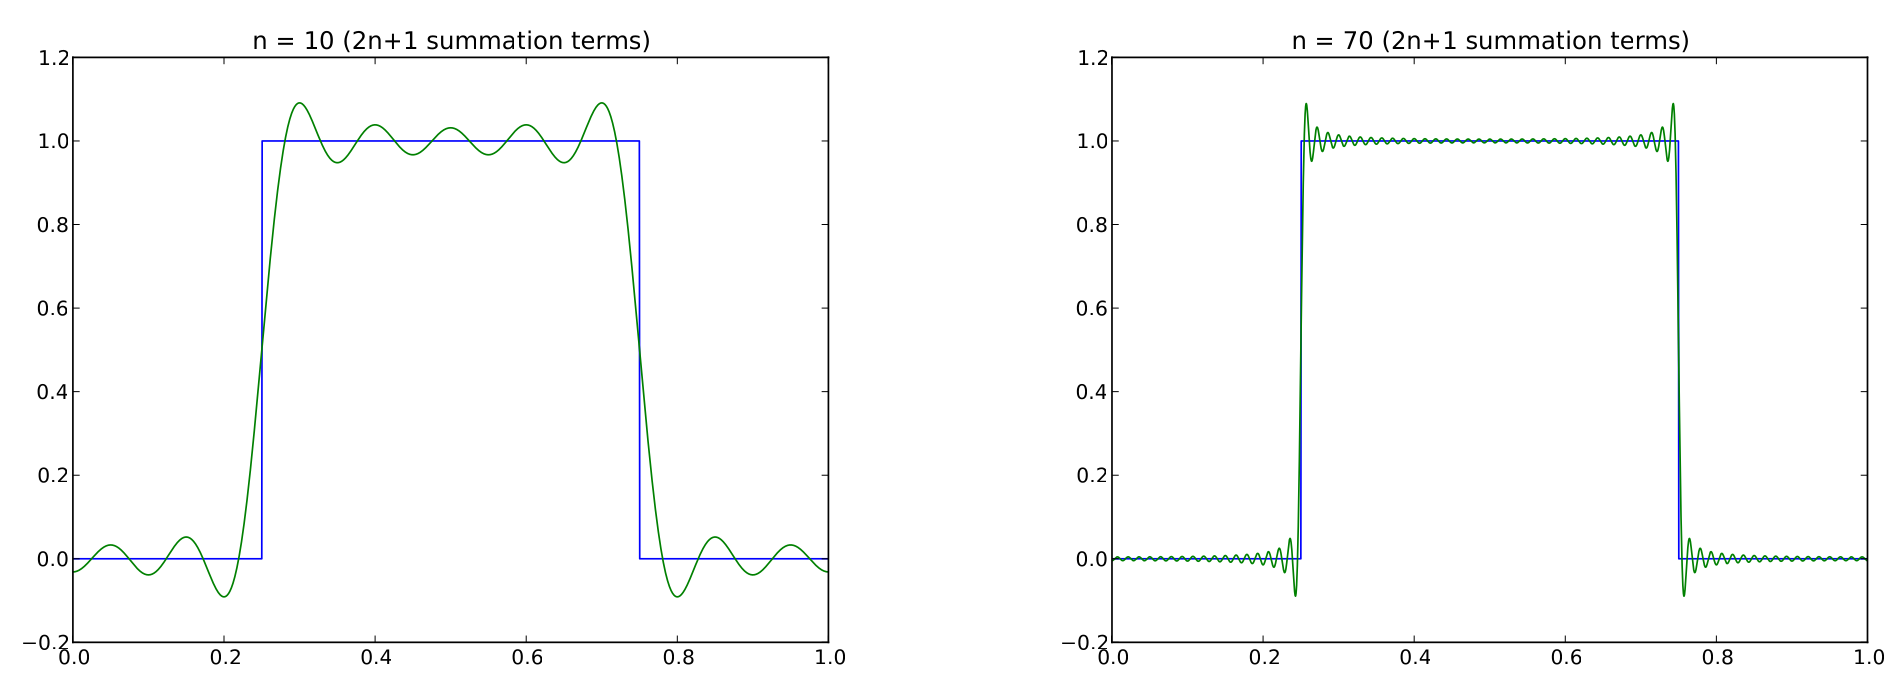
\includegraphics[width=0.95\textwidth]{assets/01_interpolation/01_trigonometric/overarcing.png}
    \end{center}
    \caption{Überschwingungen der Fourier-Reihe der charakteristischen Funktion des Intervalls $[a, b] \subseteq ]0, 1[$.
    (Abbildung aus dem Vorlesungsdokument von Prof. V. Gradinaru, Seite 69)}
    \label{fig:trigo-interp-overarcing}
\end{figure}

\stepcounter{all}
\inlineremark Meist ist es nicht möglich (oder nicht sinnvoll) die Fourier-Koeffizienten analytisch zu berechnen,
weshalb man wieder zur Numerik und der Trapezformel greift, die folgendermassen definiert ist für $t_l = \frac{l}{N}$,
wobei $l = 0, 1 \ldots, N - 1$ und $N$ die Anzahl der Intervalle ist:
\begin{align*}
    \hat{f}_N(k) := \frac{1}{N} \sum_{l = 0}^{N - 1} f(t_l) e^{-2\pi ikt_l} \approx \hat{f}(k)
\end{align*}

% TODO: Consider if we should use the below

% \begin{tikzpicture}
%     \begin{axis}[
%         legend pos=outer north east,
%         title=Function plot of $f(x)$ (parts coloured),
%         axis lines = box,
%         xlabel = $x$,
%         ylabel = $y$,
%         variable = t,
%         trig format plots = rad,
%     ]
%         \addplot [
%             domain=1:4,
%             samples=70,
%             color=blue,
%         ]
%         {log2(x)};
%         \addlegendentry{$ y=x^2 - x - 0.5$}
%     \end{axis}
%     \node (0) at (0, 0) {};
% \end{tikzpicture}


\stepcounter{subsection}
\subsection{Continuity}
\compactdef{Convergence in $\R^n$} Let $(x_k)_{k \in \N}$ where $x_k \in \R^n$ with $x_k = (x_{k, 1}, \ldots, x_{k, n})$ and let $y = (y_1, \ldots, y_n) \in \R^n$.
$(x_k)$ converges to $y$ as $k \rightarrow +\infty$ if $\forall \varepsilon > 0 \smallhspace \exists N \geq 1$ s.t. $\forall n \geq N$ we have $||x_k - y|| < \varepsilon$
% ────────────────────────────────────────────────────────────────────
\shortlemma $(x_k)$ converges to $y$ as $k \rightarrow +\infty$ iff one of following equiv. statements holds:
\bi{(1)} $\forall 1 \leq i \leq n$, the sequence $(x_{k, i})$ with $x_{k, i} \in \R$ converges to $y_i$
\bi{(2)} $(||x_k - y||)$ converges to $0$ as $k \rightarrow +\infty$
% ────────────────────────────────────────────────────────────────────
\compactdef{Continuity} Let $X \subseteq \R^n$ and $f: X \rightarrow \R^m$.
\bi{(1)} Let $x_0 \in X$. $f$ continuous in $\R^n$ if $\forall \varepsilon > 0 \smallhspace \exists \delta > 0$ s.t. if $x \in X$ satisfies $||x - x_0|| < \delta$,
then $||f(x) - f(x_0)|| < \varepsilon$
\bi{(2)} $f$ continuous \textit{on} $X$ if continuous at $x_0 \smallhspace \forall x_0 \in X$
% ────────────────────────────────────────────────────────────────────
\shortproposition Let $X$ and $f$ as prev. Let $x_0 \in X$. $f$ continuous at $x_0$ iff $\forall (x_k)_{k \geq 1}$ in $X$ s.t.
$x_k \rightarrow x_0$ as $k \rightarrow +\infty$, $(f(x_k))_{k \geq 1}$ in $\R^m$ converges to $f(x)$\\
% ────────────────────────────────────────────────────────────────────
\compactdef{Limit} Let $X$, $f$ and $x_0$ as prev. and $y \in \R^m$. $f$ \textit{has limit} $y$ as $x \rightarrow x_0$ with $x \neq x_0$ if
$\forall \varepsilon > 0 \smallhspace \exists \delta > 0$ s.t. $\forall x \neq x_0 \in X, ||x - x_0|| < \delta$ we have $||f(x) - y|| < \varepsilon$.
We write $\lim_{\elementstack{x \rightarrow x_0}{x \neq x_0}} f(x) = y$
\shortremark Also possible without ass. that $x_0 \in X$
% ────────────────────────────────────────────────────────────────────
\shortproposition Let $X$, $f$, $x_0$ and $y$ as prev. We have $\lim_{\elementstack{x \rightarrow x_0}{x \neq x_0}} f(x) = y$ 
iff $\forall (x_k)$ in $X$ s.t. $x_k \rightarrow x$ as $k \rightarrow +\infty$ and $x_k \neq x_0$ $(f(x_k))$ in $\R^m$ converges to $y$
\stepLabelNumber{all}
\shortproposition Let $X \subseteq \R^n$, $y \subseteq \R^m$, $p \in \N$ and let $f: X \rightarrow Y$ and $g: Y \rightarrow \R^p$ be cont. Then $g \circ f$ is continuous

\subsubsection{Konstruktion}

\fancydef{Trigonometrische Basis} $\{v_0, v_{N-1}\}$ ist eine Basis von $\mathbb{C}^N$, wobei $v_k = \begin{bmatrix}
    \omega_N^{0\cdot k} \\ \omega_N^{1\cdot k}1 \\ \vdots \\ \omega_N^{(N-1)\cdot k}
\end{bmatrix} \in \mathbb{C}^N$ 

Die symmetrische, nicht hermitesche Matrix $V = [v_0,\ \ldots\ , v_{N-1}]$ ist dann eine orthogonale Basis für $\mathbb{C}^N$: $V^HV = N\cdot I_N$.

Ebenfalls ist $V$ die Basiswechsel Matrix Trigonometrische Basis ($z$) $\mapsto$ Standardbasis ($y$). Algebraisch:
\begin{align*}
    y = Vz \implies z = V^{-1}y = \frac{1}{N}V^Hy = \frac{1}{N}\underbrace{F_N}_{:= V^H} y
\end{align*}

\fancydef{Fourier-Matrix} $F_N := V^H = \begin{bmatrix}
    \omega_N^0 & \omega_N^0 & \cdots & \omega_N^0 \\
    \omega_N^0 & \omega_N^1 & \cdots & \omega_N^{N-1} \\
    \omega_N^0 & \omega_N^2 & \cdots & \omega_N^{2(N-1)} \\
    \vdots     & \vdots     &        & \vdots \\
    \omega_N^0 & \omega_N^{N-1} &\cdots & \omega_N^{(N-1)^2} 
\end{bmatrix}
= \begin{bmatrix}
    \omega_N^{jk}
\end{bmatrix}^{N-1}_{j,k = 0} \in \mathbb{C}^N
$

\fancydef{Diskrete Fourier Transformation} $\mathcal{F}_N: \mathbb{C} \to \mathbb{C}$ s.d. $\mathcal{F}_N(y) = F_N y$
\subsubsection{DFT in Numpy}

Sei $y$ in der Standardbasis, und $c = \mathcal{F}_N(y)$, also $y$ in der trig. Basis.
\begin{align*}
    c = F_N \times y = \texttt{fft}(y)\quad \text{\textit{(DFT in numpy)}} & y = \frac{1}{N}F_N^Hc = \texttt{ifft}(c)\quad \textit{(Inverse DFT in numpy)}
\end{align*}

Um zur ursprünglichen Darstellung des trig. Polynoms zurück zu kommen, müssen wir die Koeffizienten umsortieren: \\
Seien $z = \frac{1}{N} F_N y$ und  $\zeta = \verb|fft.fftshift|(z)$.
\begin{align*}
    f(x) \approx \underbrace{\sum_{k=-N/2}^{N/2-1} \zeta_k \cdot e^{2 \pi ikx} }_{\text{Form des trig. Polynoms}}
\end{align*}
\setcounter{all}{13}
\inlineremark Man kann mit dieser Approximation einfach die $L^2$-Norm und Ableitungen berechnen:
\vspace{-1.5pc}
\begin{multicols}{2}
    \begin{align*}
        ||f||^2_{L^2} \approx \left\Vert \sum_{k=-N/2}^{N/2-1} \zeta_k \cdot e^{2 \pi ikx} \right\Vert^2_{L^2} = \sum_{k=-N/2}^{N/2-1} |\zeta_k|^2 = \Vert z \Vert^2_{L^2}
    \end{align*}

    \newcolumn

    \begin{align*}
        f'(t) \approx \sum_{k=-N/2}^{N/2-1} (2\pi ik) \zeta_k \cdot e^{2 \pi ikx}
    \end{align*}
\end{multicols}

\newpage
\subsection{DFT \& Lineare Algebra}

\setcounter{all}{25}
\fancydef{Zirkulant} Für einen vektor $c \in \mathbb{R}^N$ hat der Zirkulant $C \in \mathbb{R}^{N \times N}$ die Form:
\begin{align*}
    C = \begin{bmatrix}
        c_0 & c_{N-1} & c_{N-2} & \cdots & c_3 & c_2 & c_1 \\
        c_1 & c_0     & c_{N-1} & \cdots & c_4 & c_3 & c_2 \\
        c_2 & c_1     & c_{0}   & \cdots & c_5 & c_4 & c_3 \\
        \vdots & \vdots & \vdots & \ddots & \vdots & \vdots & \vdots \\
        c_{N-3} & c_{N-4} & c_{N-5} & \cdots & c_0 & c_{N-1} & c_{N-2} \\
        c_{N-2} & c_{N-3} & c_{N-4} & \cdots & c_{1} & c_0 & c_{N-1} \\
        c_{N-1} & c_{N-2} & c_{N-3} & \cdots & c_{2} & c_1 & c_0
    \end{bmatrix}
    \quad \quad \quad 
    S_N = \begin{bmatrix}
        0 & 0 & \cdots & \cdots & 0 & 1 \\
        1 & 0 & \cdots & \cdots & 0 & 0 \\
        \vdots & \vdots & \ddots & \ddots & \vdots & \vdots \\
        0 & 0 & \cdots & \cdots & 0 & 0 \\
        0 & 0 & \cdots & \cdots & 1 & 0 
    \end{bmatrix}
\end{align*}

Die Shift Matrix $S_N$ ist der Zirkulant für $c=e_2$. $S_N$ ist eine Permutationsmatrix, die alle Einträge nach vorne schiebt.
\begin{align*}
    S_N \begin{bmatrix}
        x_0 \\
        x_1 \\
        \vdots \\
        x_{N-1}
    \end{bmatrix}
    =
    \begin{bmatrix}
        x_{N-1} \\
        x_0 \\
        \vdots \\
        x_{N-2}
    \end{bmatrix}
    \quad \quad \quad 
    S_N^\top \begin{bmatrix}
        x_{N-1} \\
        x_0 \\
        \vdots \\
        x_{N-2}
    \end{bmatrix}
    =
    \begin{bmatrix}
        x_0 \\
        x_1 \\
        \vdots \\
        x_{N-1}
    \end{bmatrix}
\end{align*}

Die Shift-Matrix hat einen speziellen Bezug zu den Spaltenvektoren $v_k$ von $F_N$, und auch allen anderen Zirkulanten $C$.

\inlineremark Der $k$-te Fourier-vektor $v_k$ ist ein Eigenvektor von $S_N$ zu $\lambda_k = e^{2\pi i \frac{k}{N}}$.

\fancytheorem{Diagonalisierung von Zirkulanten} Die Eigenvektoren von $S_N$ diagonalisieren jeden Zirkulanten $C$, und sind d.h. auch die Eigenvektoren von $C$.
Die Eigenwerte erhält man aus $p(z) = c_0z^0 + \ldots + c_{N-1}z^{N-1}$.

Eine Operation mit vielen Anwendungen ist die Faltung. Sie hat einige Beziehungen zur Fourier-Transformation.

\fancydef{Faltung} $a * b := (c_k)_{k \in \mathbb{Z}} = \displaystyle\sum_{n=-\infty}^{\infty}a_nb_{k-n}$, wobei $(a_k)_{k \in \mathbb{Z}}$, $(b_k)_{k \in \mathbb{Z}}$ unendliche Folgen sind.

Die Faltung von $a = [a_0,\ldots,a_{N-1}]^\top, b = [b_0,\ldots,b_{N-1}]^\top$ ist leicht: Man erweitert beide Vektoren mit Nullen.

% ^ This needs an example

\fancydef{Zyklische Faltung} Für $N$-periodische Folgen oder Vektoren der Länge $N$:
\begin{align*}
    c = a \circledast b\quad\quad \text{s.d. } \sum_{n=0}^{N-1} a_nb_{k-n} \equiv_N \sum_{n=0}^{N-1}b_na_{n-k}
\end{align*}

\setcounter{all}{32}
\inlineremark Zyklische Faltungen von Vektoren kann man mit Zirkulanten berechnen. 
\begin{align*}
    c = a \circledast b = Ab = \underbrace{\begin{bmatrix}
        a_0 & \cdots & a_{N-1} \\
        \vdots & \ddots & \vdots \\
        a_{N-1} & \cdots & a_0
    \end{bmatrix}}_{\text{Zirkulant von } a}
    b
\end{align*}

% NOTE: I'm not sure if this below is correct. This is how I interpret what is written in the script

\setcounter{all}{30}
\inlineremark Eine Multiplikation von Polynomen $g,h$ entspricht einer Faltung im Frequenzbereich.
\begin{align*}
    \mathcal{F}_N(\underbrace{g * h}_{\text{Standard Basis}}) = \underbrace{\mathcal{F}_N(g) \cdot \mathcal{F}_N(h)}_{\text{Trigonometrische Basis}}
\end{align*}
Im Fall von $T$-periodischen Funktionen gilt: $(g * h)(x) = \frac{1}{T}\displaystyle\int_{0}^{T}g(t)h(x-t)$.

\inlineremark Da $F_N$ jeden Zirkulant $C$ diagonalisiert (Satz 3.4.27), gilt sogar:
\begin{align*}
    c = a \circledast b = Ab = F_N^{-1}p(D)F_Nb \quad \quad \quad (p(D) \text{ ist Diagonalmatrix der } \lambda \text{ von } C )
\end{align*}
Man erhält so letzendlich das Faltungs-Theorem: Die $F_N$-Transformierte einer Faltung ist genau das gleiche wie die Multiplikation zweier $F_N$-Transormierten. Da die DFT in $\mathcal{O}(n\log(n))$ (Kap. 3.5) geht, gilt dies nun auch für die Faltung.
\begin{align*}
    F_Nc = \text{diag}(F_N a) F_N b
\end{align*}
% ┌                                                ┐
% │     AUTHOR: Janis Hutz<info@janishutz.com>     │
% └                                                ┘

\newsection
\subsection{Schnelle Fourier Transformation}
Da es viele Anwendungen für die Fourier-Transformation gibt, ist ein Algorithmus mit guter Laufzeit sehr wichtig.
Während eine naive version des DFT-Algorithmus eine Laufzeit von $\tco{N^2}$ hat,
so hat der Fast Fourier Transform Algorithmus nur eine Laufzeit von $\tco{N \log(N)}$,
was bei $N = 1024$ bereits eine Laufzeitsverbesserung von $100\times$ mit sich bringt ($\tco{10\,000}$ vs $\tco{1\,000\,000}$ Operationen)!
Die untenstehende Abbildung \ref{fig:trigo-interp-fft-runtimes} findet sich, zusammen mit dem Code,
mit der sie produziert wurde im Skript auf Seite 86-88

\setLabelNumber{all}{3}
\begin{figure}[h!]
    \begin{center}
        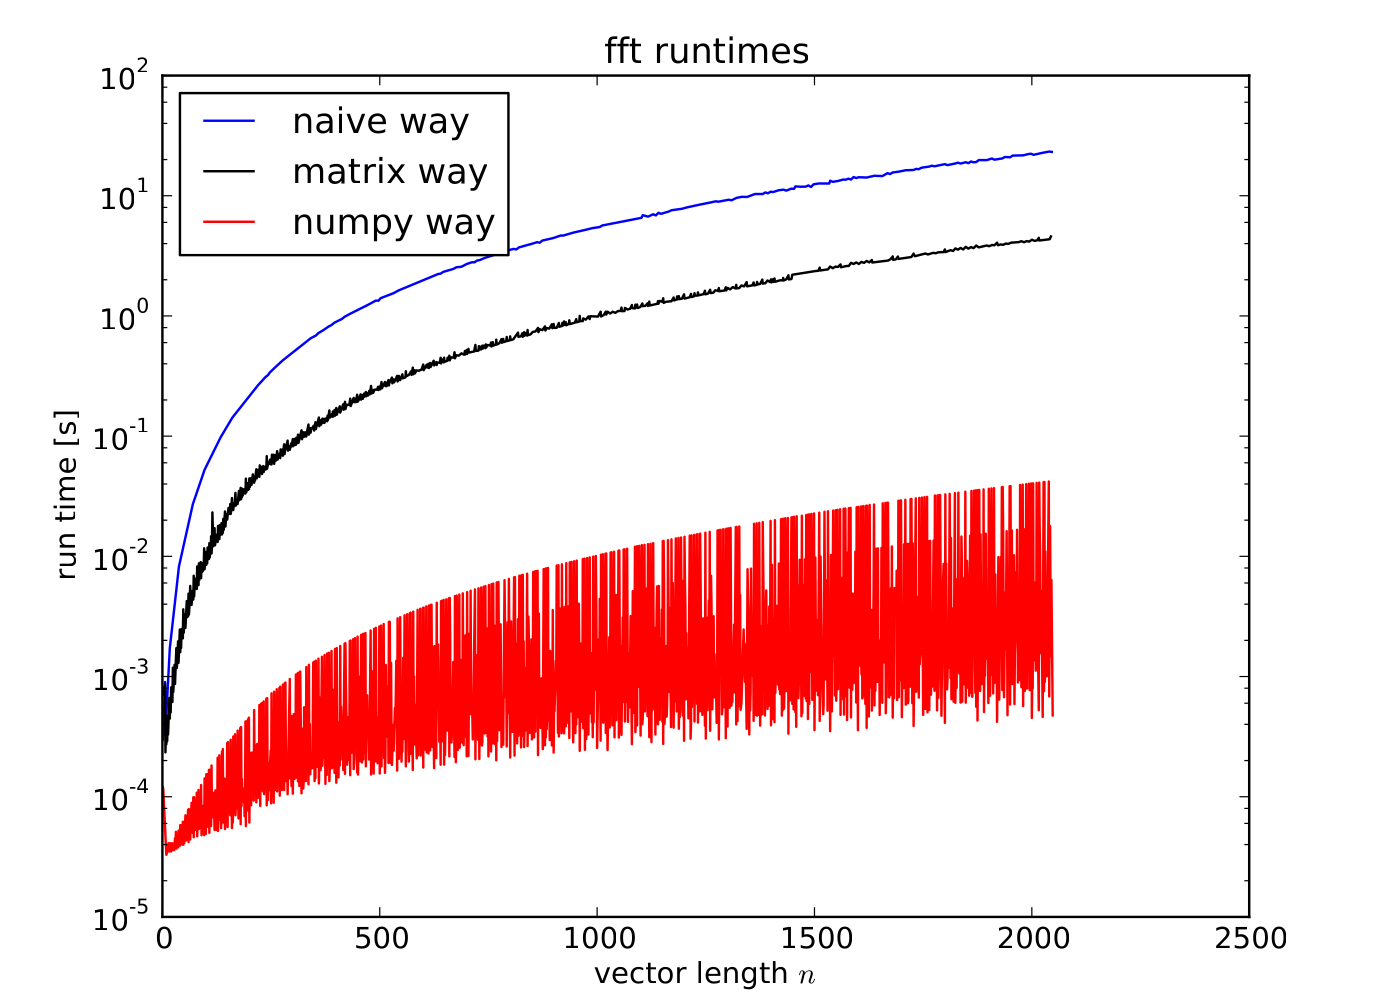
\includegraphics[width=0.7\textwidth]{assets/01_interpolation/01_trigonometric/fft-runtimes.png}
    \end{center}
    \caption{Vergleich der Laufzeit von verschiedenen Fourier-Transformations-Algorithmen.
    (Abbildung 3.3.3 aus dem Vorlesungsdokument von Prof. V. Gradinaru, Seite 88)}
    \label{fig:trigo-interp-fft-runtimes}
\end{figure}

Der hier besprochene Cooley-Tukey-Algorithmus wurde ursprünglich von Gauss 1805 entdeckt, dann vergessen und schliesslich 1965 von Cooley und Tukey wiederentdeckt.
Der Algorithmus verwendet einen ``Divide and Conquer'' Approach, also ist logischerweise die Idee,
dass man die Berechnung einer DFT der Länge $n$ auf die Berechnung vieler DFTs kleinerer Längen zurückführen kann.

Für den Algorithmus müssen folgende vier Optionen betrachtet werden:
\begin{enumerate}[label=\Roman*]
    \item Vektoren der Länge $N = 2m \Longrightarrow$ Laufzeit gut
    \item Vektoren der Länge $N = 2^L \Longrightarrow$ Laufzeit ideal
    \item Vektoren der Länge $N = pq$ mit $p, q \in \Z \Longrightarrow$ Etwas langsamer
    \item Vektoren der Länge $N$, mit $N$ prim $\Longrightarrow$ ca. $\tco{N^2}$, besonders für $N$ gross
\end{enumerate}
Wir formen die Fourier-Transformation um für den ersten Fall ($N = 2m$):
\rmvspace
\begin{align*}
    c_k & = \sum_{j = 0}^{N - 1} y_j e^{- \frac{2\pi i}{N} jk}                                                                     \\
        & = \sum_{j = 0}^{m - 1} y_{2j} e^{-\frac{2 \pi i}{N}2jk} + \sum_{j = 0}^{m - 1} y_{2j + 1} e^{-\frac{2\pi i}{N}(2j + 1)k} \\
        & = \sum_{j = 0}^{m - 1} \left( y_{2j} e^{-\frac{2 \pi i}{N \div 2}jk} \right)
    + e^{- \frac{2\pi}{N} k} \left( \sum_{j = 0}^{m - 1} y_{2j + 1} e^{-\frac{2\pi i}{N \div 2}jk} \right)
\end{align*}
Der zweite Fall ist einfach eine rekursive Weiterführung des ersten Falls,
bei welchem dann das $m$ kontinuierlich weiter dividiert wird bis zum Trivialfall mit einer $1 \times 1$-Matrix.

\innumpy gibt es die Funktionen \texttt{np.fft.fft} (Vorwärts FFT), \texttt{np.fft.ifft} (Rückwärts FFT). 
\texttt{scipy.fft} liefert dieselben Funktionen und sie sind oft etwas schneller als die von \texttt{numpy}

\stepcounter{subsection}
\subsection{Continuity}
\compactdef{Convergence in $\R^n$} Let $(x_k)_{k \in \N}$ where $x_k \in \R^n$ with $x_k = (x_{k, 1}, \ldots, x_{k, n})$ and let $y = (y_1, \ldots, y_n) \in \R^n$.
$(x_k)$ converges to $y$ as $k \rightarrow +\infty$ if $\forall \varepsilon > 0 \smallhspace \exists N \geq 1$ s.t. $\forall n \geq N$ we have $||x_k - y|| < \varepsilon$
% ────────────────────────────────────────────────────────────────────
\shortlemma $(x_k)$ converges to $y$ as $k \rightarrow +\infty$ iff one of following equiv. statements holds:
\bi{(1)} $\forall 1 \leq i \leq n$, the sequence $(x_{k, i})$ with $x_{k, i} \in \R$ converges to $y_i$
\bi{(2)} $(||x_k - y||)$ converges to $0$ as $k \rightarrow +\infty$
% ────────────────────────────────────────────────────────────────────
\compactdef{Continuity} Let $X \subseteq \R^n$ and $f: X \rightarrow \R^m$.
\bi{(1)} Let $x_0 \in X$. $f$ continuous in $\R^n$ if $\forall \varepsilon > 0 \smallhspace \exists \delta > 0$ s.t. if $x \in X$ satisfies $||x - x_0|| < \delta$,
then $||f(x) - f(x_0)|| < \varepsilon$
\bi{(2)} $f$ continuous \textit{on} $X$ if continuous at $x_0 \smallhspace \forall x_0 \in X$
% ────────────────────────────────────────────────────────────────────
\shortproposition Let $X$ and $f$ as prev. Let $x_0 \in X$. $f$ continuous at $x_0$ iff $\forall (x_k)_{k \geq 1}$ in $X$ s.t.
$x_k \rightarrow x_0$ as $k \rightarrow +\infty$, $(f(x_k))_{k \geq 1}$ in $\R^m$ converges to $f(x)$\\
% ────────────────────────────────────────────────────────────────────
\compactdef{Limit} Let $X$, $f$ and $x_0$ as prev. and $y \in \R^m$. $f$ \textit{has limit} $y$ as $x \rightarrow x_0$ with $x \neq x_0$ if
$\forall \varepsilon > 0 \smallhspace \exists \delta > 0$ s.t. $\forall x \neq x_0 \in X, ||x - x_0|| < \delta$ we have $||f(x) - y|| < \varepsilon$.
We write $\lim_{\elementstack{x \rightarrow x_0}{x \neq x_0}} f(x) = y$
\shortremark Also possible without ass. that $x_0 \in X$
% ────────────────────────────────────────────────────────────────────
\shortproposition Let $X$, $f$, $x_0$ and $y$ as prev. We have $\lim_{\elementstack{x \rightarrow x_0}{x \neq x_0}} f(x) = y$ 
iff $\forall (x_k)$ in $X$ s.t. $x_k \rightarrow x$ as $k \rightarrow +\infty$ and $x_k \neq x_0$ $(f(x_k))$ in $\R^m$ converges to $y$
\stepLabelNumber{all}
\shortproposition Let $X \subseteq \R^n$, $y \subseteq \R^m$, $p \in \N$ and let $f: X \rightarrow Y$ and $g: Y \rightarrow \R^p$ be cont. Then $g \circ f$ is continuous

\newpage
\subsubsection{Zero-Padding-Auswertung}
Ein trigonometrisches Polynom $p_{N - 1}(t)$ kann effizient an den äquidistanten Punkten $\frac{k}{M}$ mit $M > N$ ausgewertet werden, für $k = 0, \ldots, M - 1$.
Dazu muss das Polynom $p_{N - 1} \in \mathcal{T}_N \subseteq \mathcal{T}_M$ in der trigonometrischen Basis $\mathcal{T}_M$ neugeschrieben werden,
in dem man \bi{Zero-Padding} verwendet, also Nullen im Koeffizientenvektor an den Stellen höheren Frequenzen einfügt.

\TODO Insert cleaned up code from Page 95 (part of exercises)

% ┌                                                ┐
% │     AUTHOR: Janis Hutz<info@janishutz.com>     │
% └                                                ┘

\newsection
\subsection{Fehlerabschätzungen}

\begin{definition}[]{Konvergenz}
    \begin{multicols}{2}
        \fhl{Algebraische Konvergenz}\\
        Wenn der Fehler $E(n) = \tco{\frac{1}{n^p}}$ mit $p > 0$ ist

        \fhl{Exponentielle Konvergenz}\\
        Wenn der Fehler $E(n) = \tco{q^n}$ mit $0 \leq q < 1$
    \end{multicols}
\end{definition}

\inlineex Zur Fehlerbetrachtung verwenden wir drei Funktionen $f : [0, 1] \rightarrow \R$, welche wir mit trigonometrischer Interpolation an den Punkten $\frac{k}{N}$ approximieren:
\begin{enumerate}[label=(\Roman*)]
    % FIXME: Possibly wrong function definition in script
    \item Stufenfunktion (periodische Fortsetzung von $f$) $f : [0, 1] \rightarrow \R$ mit $f(t) = \begin{cases}
                  0 & \text{für } \left| t - \frac{1}{2} \right| > \frac{1}{4}    \\
                  1 & \text{für } \left| t - \frac{1}{2} \right| \leq \frac{1}{4}
              \end{cases}$
    \item Periodische, glatte Funktion $h: \R \rightarrow \R$ mit $h(t) = \displaystyle \frac{1}{\sqrt{1 + \frac{1}{2} \sin(2\pi t)}}$
          % TODO: Is it $h$ or $g$ here? $g$ makes little sense imho
    \item Hutfunktion (periodische Fortsetzung von $h$) $g : [0, 1] \rightarrow \R$ mit $g(t) = \left| t - \frac{1}{2} \right|$
\end{enumerate}
Die untenstehende Abbildung \ref{fig:interpolation-error-examples} beinhaltet einen Plot, auf dem die Konvergenz in Abhängigkeit des Grades des Interpolationspolynoms aufgetragen ist.

\begin{figure}[h!]
    \begin{center}
        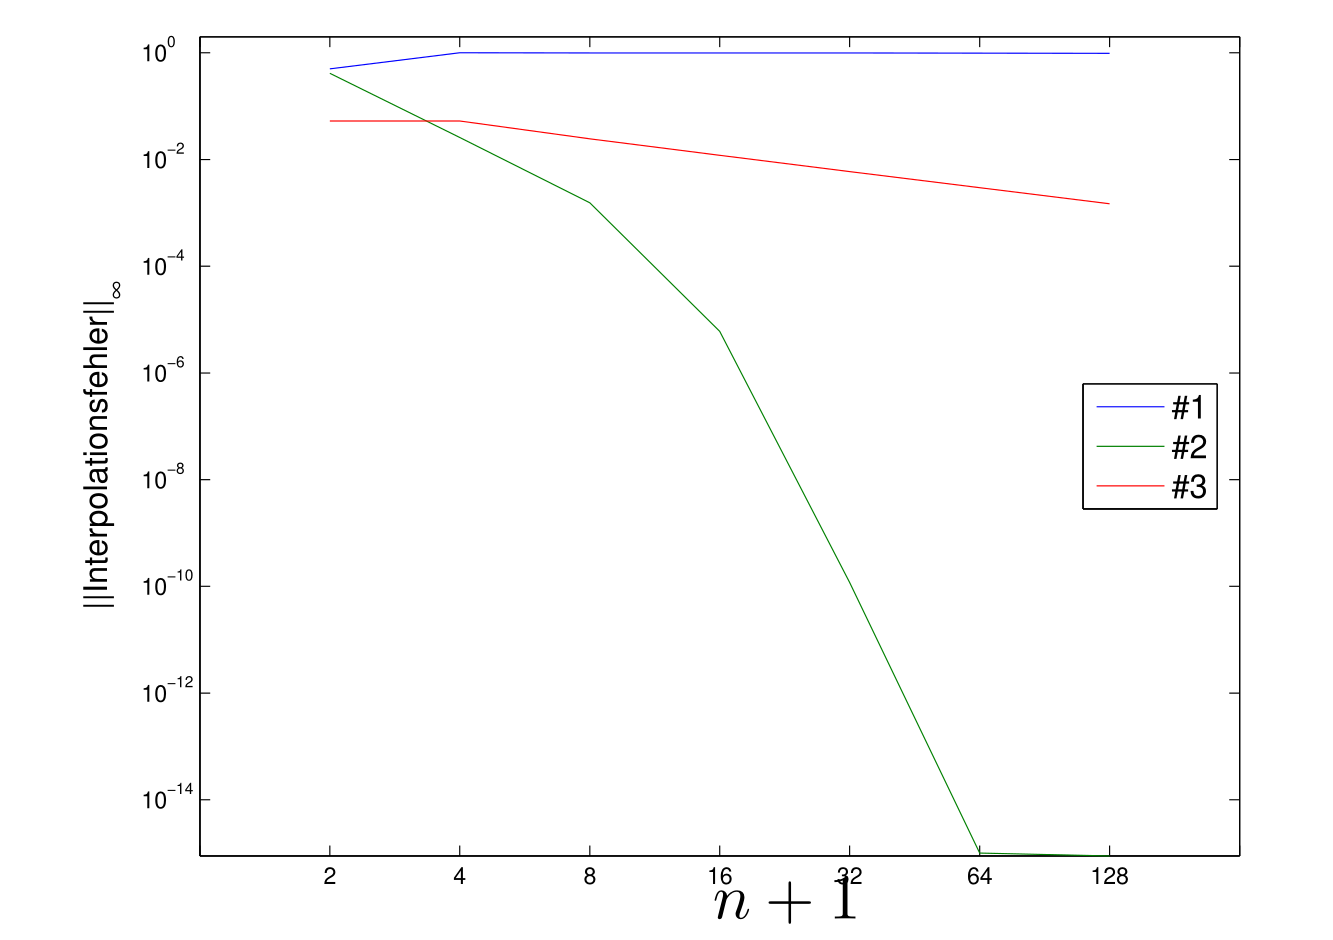
\includegraphics[width=0.6\textwidth]{assets/01_interpolation/01_trigonometric/interpolation-error-examples.png}
    \end{center}
    \caption{Interpolierungsfehler der Beispiele. Algebraische Konvergenz für (I) und (III), exponentielle für (II).
    (Abbildung 3.5.2 aus dem Vorlesungsdokument von Prof. V. Gradinaru, Seite 96)}
    \label{fig:interpolation-error-examples}
\end{figure}
Auch hier tritt das Gibbs-Phänomen wieder an den Sprungstellen von $f(t)$ auf.
Dies verursacht die Verlangsamung der Konvergenz in den Stellen, in welchen die Funktion nicht glatt ist.

\newpage
\stepLabelNumber{all}
\inlineex Sei für $\alpha \in [0, 1)$ $\displaystyle f(t) = \frac{1}{\sqrt{1 - \alpha \sin(2\pi t)}}$.
Die Konvergenz ist exponentiell in $n$ und je kleiner $\alpha$, desto schneller ist sie.
In der untenstehenden Abbildung \ref{fig:interpolation-error-convergence} sind einige Beispiele aufgetragen:
\begin{figure}[h!]
    \begin{center}
        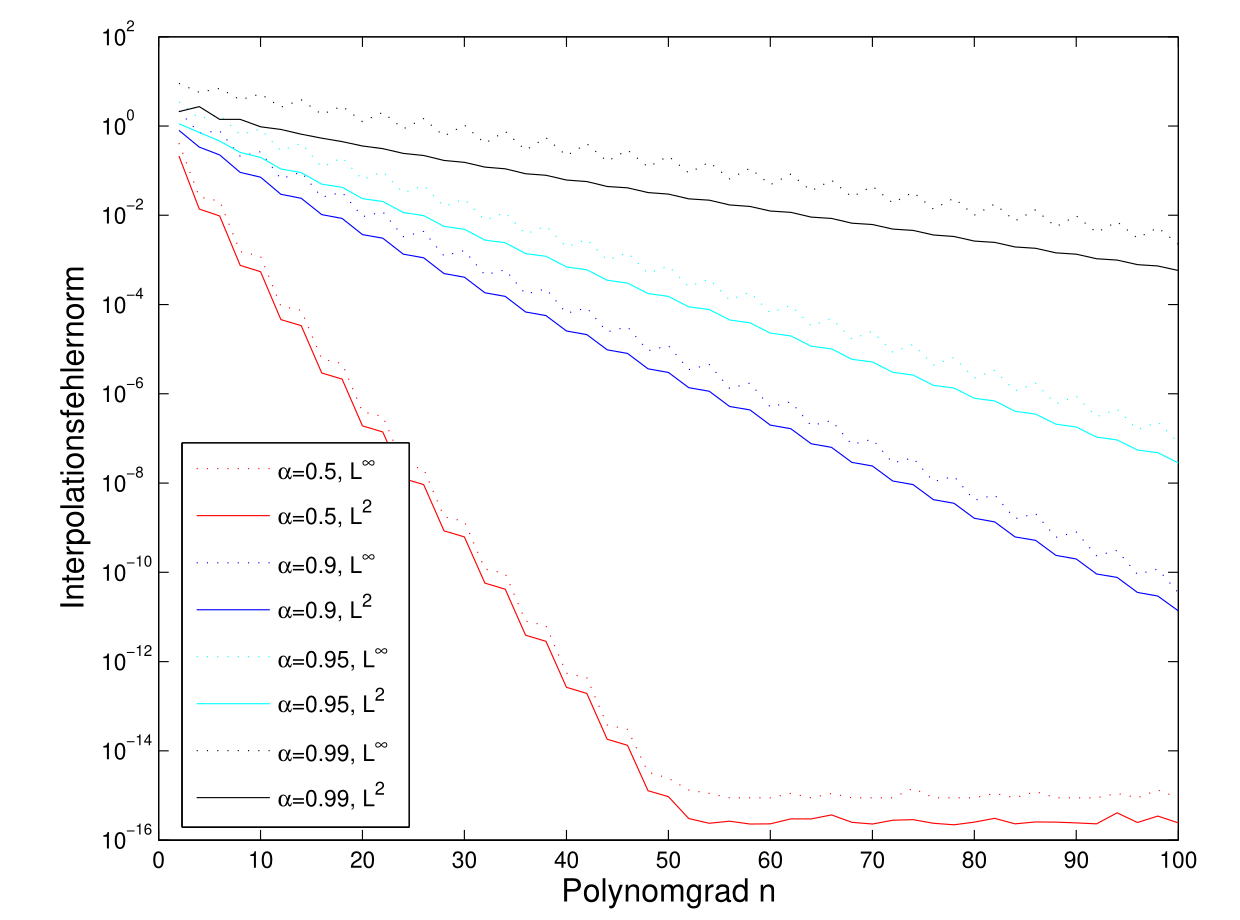
\includegraphics[width=0.6\textwidth]{assets/01_interpolation/01_trigonometric/interpolation-error-convergence.png}
    \end{center}
    \caption{Fehler bei der trigonometrischen Interpolation.
    (Abbildung 3.5.5 aus dem Vorlesungsdokument von Prof. V. Gradinaru, Seite 98)}
    \label{fig:interpolation-error-convergence}
\end{figure}


\setLabelNumber{all}{6}
\begin{theorem}[]{Aliasing}
    Der k-te Fourier-Koeffizient des $N$-ten trigonometrischen Interpolationspolynoms unterscheidet sich vom $k$-ten Fourier-Koeffizienten von $f$ 
    gerade um die Summe aller Fourier-Koeffizienten, die um ganze Vielfache von $N$ vom $k$-ten Fourier-Koeffizienten verschoben sind:
    \begin{align*}
        \hat{p}_N(k) - \hat{f}(k) = \sum_{j \neq 0 \in \Z} \hat{f}(k + jN)
    \end{align*}
\end{theorem}
% FIXME: On page 98, just below the above theorem, there is a text I have no idea what he meant to say... in all honesty, I don't think he was sober when he wrote that

\inlinecorollary Für $f \in \C^p([0, 1])$ mit $p \geq 1$ und $f$ $1$-periodisch, dann gilt: $|\hat{p}_N(k) - \hat{f}(k)| = \tco{(N^{-p})}$ für $|k| \leq \frac{N}{2}$

Das heisst also, dass die Fourier-Koeffizienten von $f$ bei kleinen Frequenzen $\left( \text{hier } |k| < \frac{N}{2} \right)$
sehr gut durch die Fourier-Koeffizienten des trigonometrischen Interpolationspolynoms approximiert werden.

\begin{theorem}[]{Fehler der trigonometrischen Interpolation}
    Falls $f$ $1$-periodisch ist und die Reihe $\sum_{k \in \Z} |\hat{f}(k)|$ absolut konvergiert, dann ist der Approximationsfehler definiert als:
    \begin{align*}
        |p_N(x) - f(x)| \leq 2 \sum_{|k| \geq \frac{N}{2}} |\hat{f}(k)| \mediumhspace \forall x \in \R
    \end{align*}
\end{theorem}
Da durch diesen Satz die obere Schranke für den Approximationsfehler durch die schwer approximierbaren Fourier-Koeffizienten $\hat{f}(k)$ gegeben ist,
heisst das folgendes für die Approximation von Polynomen von Grad $\deg(P(x)) < n$ für unser Approximationspolynom von Grad $\deg(P_N(x)) = n$:

\fancycorollary{Abtasttheorem} Sei $f$ $1$-periodisch mit maximaler Frequenz $m$, also $\hat{f}(k) = 0 \smallhspace \forall |k| > m$. Falls $N > 2m$, dann gilt $p_N(x) = f(x) \smallhspace \forall x$

\inlineex Ein Beispiel aus der Musik: Wir haben ein analoges Signal und wollen es digitalisieren. 
Wir messen die Spannungswerte in äquidistanten Punkten. 
Falls wir jedoch die Frequenz der Messung zu niedrig wählen, so kann ein total falsches Interpolationspolynom entstehen,
wie in der untenstehenden Abbildung \ref{fig:aliasing} zu sehen:
\begin{figure}[h!]
    \begin{center}
        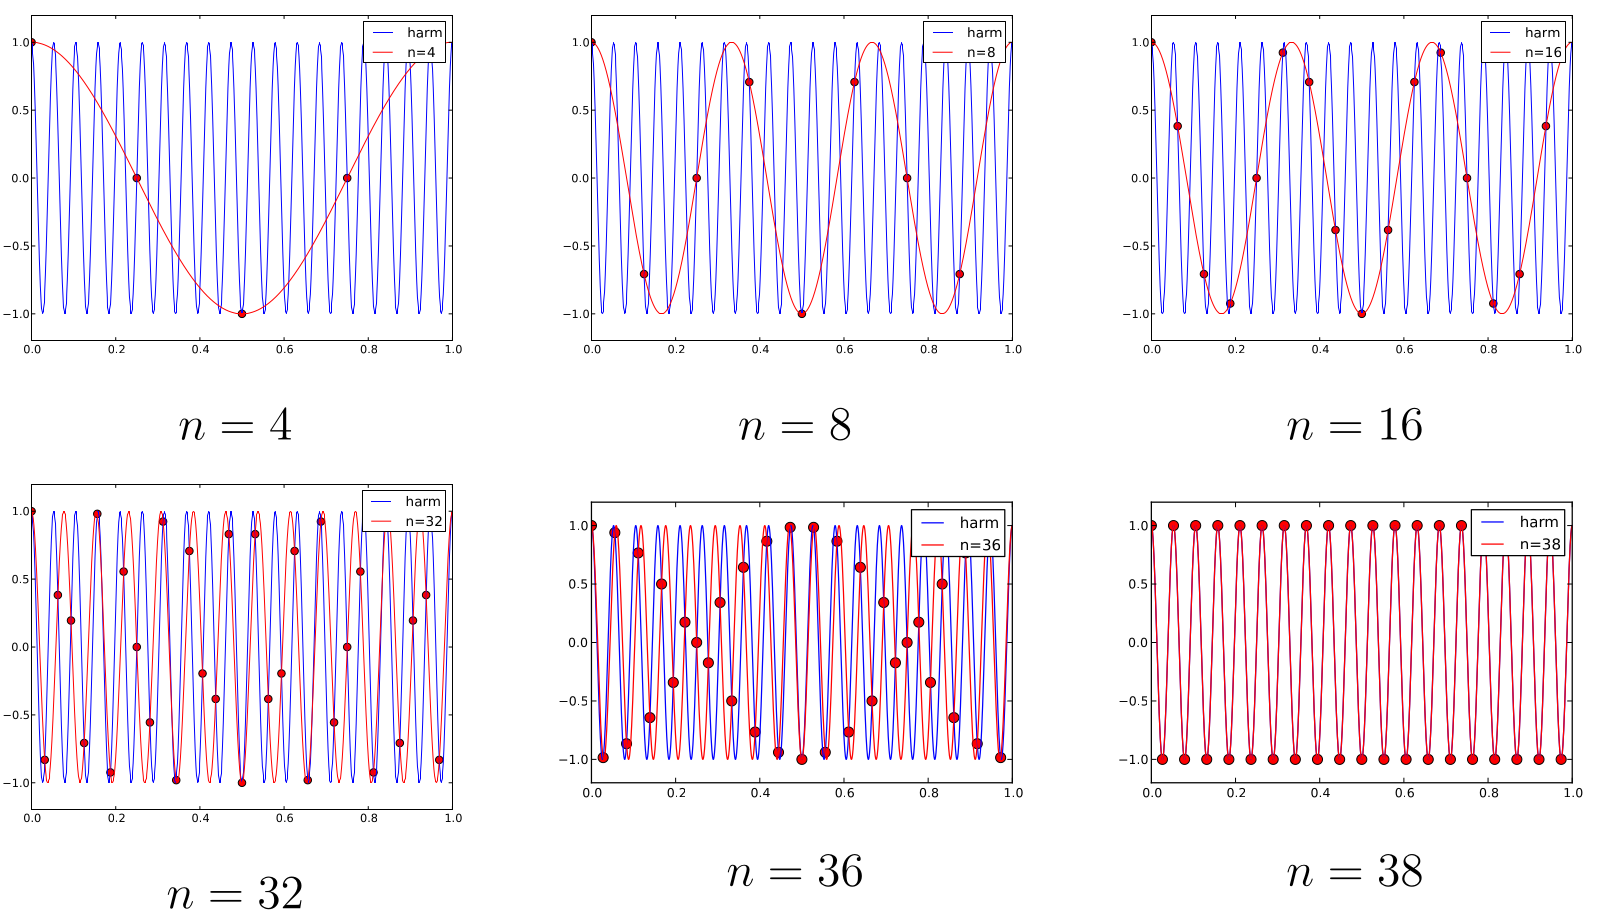
\includegraphics[width=0.95\textwidth]{assets/01_interpolation/01_trigonometric/aliasing-in-music.png}
    \end{center}
    \caption{Aliasing für $f(t) = \cos(2\pi \cdot 19t)$. (Abbildung 3.5.10 aus dem Vorlesungsdokument von Prof. V. Gradinaru, Seite 100)}
    \label{fig:aliasing}
\end{figure}
Für unser Signal bedeutet das also, dass wir eine Art Verzerrung auf der Aufnahme haben, oder für Autoräder, dass es so scheint, als würden sich die Räder rückwärts drehen.

\begin{theorem}[]{Fehlerabschätzung}
    Sei $f^{(k)} \in L^2(0, 1) \smallhspace \forall k \in \N$, dann gilt:
    \rmvspace
    \begin{align*}
        ||f - p_N(f)||_{L^2(0, 1)} \leq \sqrt{1 + c_k} N^{-k} ||f^{(k)}||_{L^2(0, 1)} \text{ wobei } c_k = 2 \sum_{l = 1}^{\infty} (2l - 1)^{-2k}
    \end{align*}
\end{theorem}
Also, je mehr Ableitungen in $L^2(0, 1)$ liegen, desto kleiner ist der Fehler.


Im Skript auf Seiten 101 und 102 gibt es einige Abbildungen die eine gewisse Intuition hinter der Approximation und den entstandenen Fehlern gibt.




\end{document}
